\documentclass[../notas medios.tex]{subfiles}

\begin{document}
\chapter{Equilibrio}

\graphicspath{{img/Cap4/}} 	% Specifies the directory where pictures are stored
\section{Introducción}

En esta sección se formularán las ecuaciones de equilibrio para un medio continuo, haciendo uso del principio de conservación de moméntum y de momento de moméntum. Estas darán como resultado un sistema de ecuaciones diferenciales parciales en las componentes del tensor de tensiones y demostrarán la simetría del tensor de tensiones. Una vez planteadas las ecuaciones, la sección concluye con el estudio de algunas soluciones\footnote{Por soluciones nos referimos a funciones de las componentes del tensor de esfuerzos que satisfacen las ecuaciones de equilibrio y las condiciones de frontera.} clásicas para el caso de sólidos.

Al final de esta sección el estudiante deberá estar en la capacidad de:

\begin{itemize}
\item[•] Identificar el dominio del problema y su frontera (o superficie).
\item[•] Reconocer la diferencia entre equilibrio local y global en un medio continuo.
\item[•] Identificar condiciones de frontera de tracciones para diferentes problemas particulares.
\item[•] Recuperar y/o verificar condiciones de frontera.
\item[•] Entender los aspectos matemáticos fundamentales del problema de valores en la frontera de la mecánica de los medios continuos en sistemas de referencia cartesianos y cilíndricos.
\item[•] Verificar si una función de tensiones es solución a un problema particular de la mecánica de los medios continuos.
\item[•] Analizar,desde el punto de vista de tensiones, algunas soluciones clásicas de la mecánica de los medios continuos.
\end{itemize}


\section{Ecuaciones de Equilibrio diferencial}
En las secciones anteriores se describió el modelo del medio continuo en términos de fuerzas.  El paso del modelo discreto al modelo continuo, vía la hipótesis fundamental de continuidad, se tradujo en un tratamiento de las fuerzas ya no como vectores sino que estas tuvieron que ser tratadas en términos de funciones tensoriales con significado de densidades de fuerza o fuerzas por unidad de superficie.  Es así como ahora en el modelo continuo el tensor de tensiones se convierte en el dispositivo matemático que produce cambios en la cantidad de movimiento en el sistema de infinitas partículas.

Nuestro siguiente objetivo es entonces el de proponer las ecuaciones que gobiernan el flujo de las densidades superficiales de fuerza $\sigma$, desde sus valores conocidos en la frontera en términos del vector de tracciones ${\vec t^{(n)}}$ , hasta cualquier punto del medio continuo.  La determinación de estas tensiones no solamente es un problema con su propio valor asociado, sino que también es el camino necesario si se desean conocer los cambios en la cantidad de movimiento del sistema.

Es esperable además, si se sabe que el modelo matemático utilizado para el tratamiento del sistema de muchas (infinitas) partículas ha sido construido a partir de las leyes de la Mecánica Newtoniana, que las ecuaciones resultantes deban estar estrechamente ligadas a estas (¿O son las mismas?).  Acá partimos entonces de los principios fundamentales de la mecánica Newtoniana.

Considerese un elemento diferencial arbitrario tomado de un medio continuo y de dimensiones $dx \times dy \times dz$ como el que se muestra en la \cref{diff}\footnote{Debe notarse que este bloque de tensiones corresponde a un elemento del continuo de tamaño diferencial, mientras que en las secciones anteriores hacíamos uso de un elemento similar pero que no tenía ningún tamaño asociado y que solo se convertía en una forma práctica de representar el estado de tensiones en un punto material en un sistema de referencia cartesiano.

Por ejemplo en aquel caso si cortábamos un punto material con un plano con dirección normal $\hat{n}$ y con vector de tracciones asociado $\vec t^{(\hat n)}$ teníamos que este vector era igual y opuesto al asociado al corte con un plano con dirección $-\hat{n}$. De esta forma se decidió representar el tensor de esfuerzos para un punto del continuo mediante los tres vectores de tracción asociados con  3 direcciones perpendiculares $\hat{\imath}$, $\hat{\jmath}$ y $\hat{k}$ y sus direcciones opuestas $-\hat{\imath}$, $-\hat{\jmath}$ y $-\hat{k}$.}

Denotemos las áreas superficiales de las caras de dicho elemento y su volumen como;
\begin{align*}
&d{S_x} = dydz\, ,\\
&d{S_z} = dxdy\, ,\\
&d{S_y} = dxdz\, ,\\
&dV = dxdydz\, .
\end{align*}

En lo que sigue nos proponemos plantear las condiciones de equilibrio del elemento como si se tratara de un cuerpo rígido. Para esto supondremos además que el elemento se encuentra sometido a la acción de fuerzas de cuerpo $\vec B = B_x \hat\imath + B_y \hat\jmath + {B_z}\hat k$.
\begin{figure}[h]
\centering
	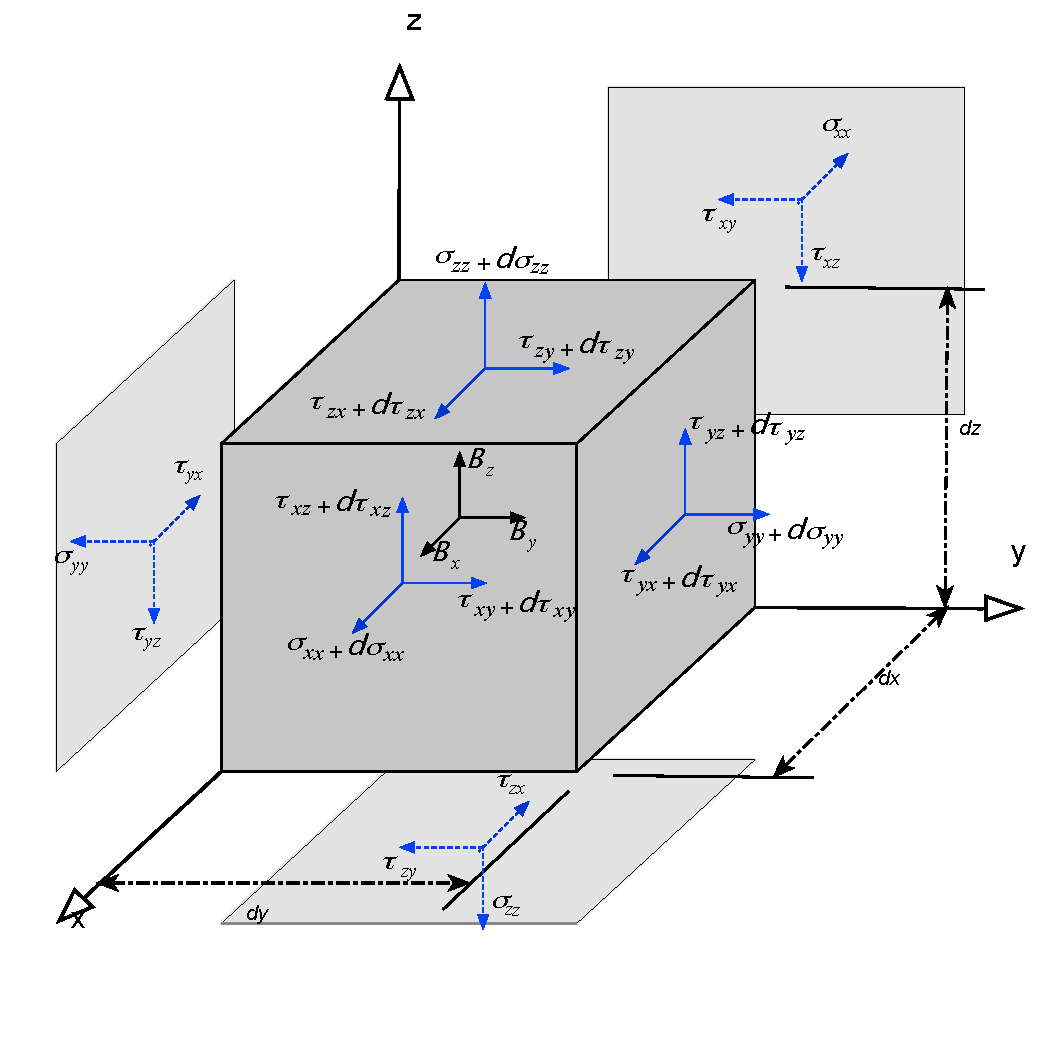
\includegraphics[width=4.0 in]{diffblock.pdf}
	\caption{Tensiones en un elemento diferencial de tamaño $dx\, dy\, dz$.}
	\label{diff}
\end{figure}

Dado que el bloque en cuestión tiene tamaño (así sea diferencial) es esperable que las tensiones sobre una cara y otra ya no permanezcan constantes sino que estas experimenten variaciones también diferenciales. Por ejemplo, si la tensión normal sobre la cara con vector $-\hat{i}$ y localizada sobre el punto O es ${\sigma _{xx}}$ entonces se tiene que la tensión normal sobre el punto $x_O+dx$ está dada por ${\sigma _{xx}} + \frac{{\partial {\sigma _{xx}}}}{{\partial x}}dx$ tal y como se muestra en la \cref{EQx}.


Con esta consideración de por medio planteamos ahora la condición de equilibrio en la dirección $x$:
\[\sum F_x = 0\, . \]

Y teniendo cuidado de convertir las tensiones a fuerzas tras considerar el área de cada cara. Apoyándonos nuevamente en la \cref{EQx} en la cual se muestran todas las tensiones en la dirección $x$ tenemos que
\begin{align*}
\left( \sigma_{xx} + \frac{\partial \sigma_{xx}}{\partial x}dx \right)d{S_x} & - {\sigma _{xx}}d{S_x} - {\tau _{yx}}d{S_y} + \left( {{\tau _{yx}} + \frac{{\partial {\tau _{yx}}}}{{\partial y}}dy} \right)d{S_y} \nonumber \\ 
&\qquad {} - {\tau _{zx}}d{S_z} + \left( {{\tau _{zx}} + \frac{{\partial {\tau _{zx}}}}{{\partial z}}dy} \right)d{S_z} + {B_x}dV = 0
\end{align*}
cancelando los términos iguales y opuestos y eliminando el diferencial de volumen común a todos los términos se tiene
\[\frac{{\partial {\sigma _{xx}}}}{{\partial x}}\cancel{dxd{S_x}} + \frac{{\partial {\tau _{yx}}}}{{\partial y}}\cancel{dyd{S_y}} + \frac{{\partial {\tau _{zx}}}}{{\partial z}}\cancel{dyd{S_z}} + {B_x}\cancel{dV} = 0\, .\]

\begin{figure}[h]
\centering
	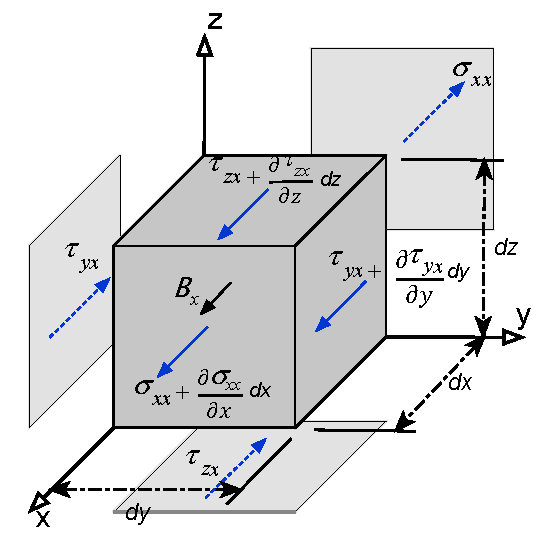
\includegraphics[width=3.0 in]{Eqx.pdf}
	\caption{Variación de las tensiones que producen fuerzas en la dirección $x$ sobre un elemento diferanecial de dimensiones $dx$, $dy$, $dz$.}
	\label{EQx}
\end{figure}




\begin{equation}
\frac{{\partial {\sigma _{xx}}}}{{\partial x}} + \frac{{\partial {\tau _{yx}}}}{{\partial y}} + \frac{{\partial {\tau _{zx}}}}{{\partial z}} + {B_x} = 0.
\label{Equil_x}
\end{equation}

La \cref{Equil_x} es una ecuación diferencial parcial que controla la variación de las componentes $\sigma_{xx}$, $\tau_{yx}$ y $\tau_{zx}$.


\subsubsection{Tarea}
Usando las condiciones de equilibrio en las direcciones $y$ y $z$ (dadas por $\sum {{F_y} = 0}$ y $\sum {{F_z} = 0}$) para los elementos diferenciales mostrados en las \cref{EQy} y \cref{EQz} demostrar que estas resultan en
\begin{align*}
&\frac{{\partial {\tau _{xy}}}}{{\partial x}} + \frac{{\partial {\sigma _{yy}}}}{{\partial y}} + \frac{{\partial {\tau _{zy}}}}{{\partial z}} + {B_y} = 0\\
&\frac{{\partial {\tau _{xz}}}}{{\partial x}} + \frac{{\partial {\tau _{yz}}}}{{\partial y}} + \frac{{\partial {\sigma _{zz}}}}{{\partial z}} + {B_z} = 0\, .
\end{align*}


\begin{figure}[H]
     \centering
     \subfloat[Fuerzas en $y$]{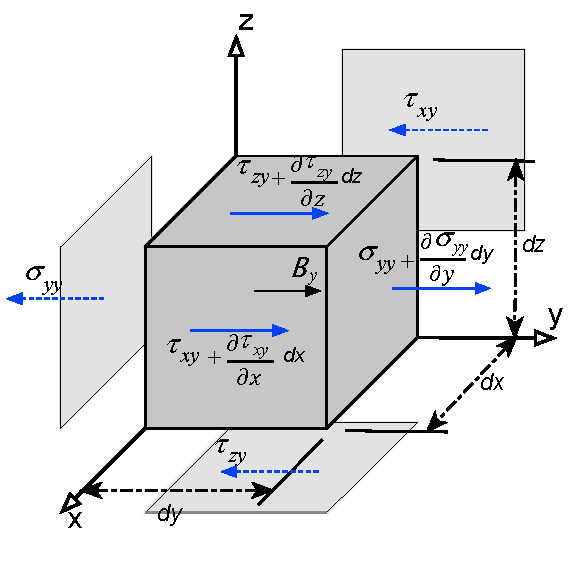
\includegraphics[width=2.8 in]{Eqy.pdf}\label{EQy}}
     \hspace{0.5cm}
     \subfloat[Fuerzas en $z$]{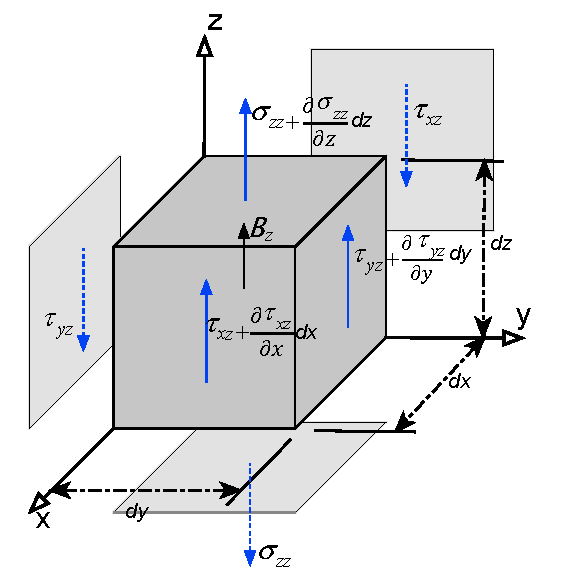
\includegraphics[width=2.8 in]{Eqz.pdf}\label{EQz}}
     \caption{Variación de las tensiones que producen fuerzas en la dirección $y$ y $z$ sobre un elemento diferencial de dimensiones $dx \times dy \times dz$.}
     \label{steady_state}
\end{figure}


Por otro lado, usando ahora las condiciones de equilibrio rotacional se tiene de la condición $\sum {{M_z} = 0}$;

\[{\tau _{yx}}d{S_y}\frac{1}{2}dy + \left( {{\tau _{yx}} + \frac{{\partial {\tau _{yx}}}}{{\partial y}}dy} \right)d{S_y}\frac{1}{2}dy - {\tau _{xy}}d{S_x}\frac{1}{2}dx - \left( {{\tau _{xy}} + \frac{{\partial {\tau _{xy}}}}{{\partial x}}dx} \right)d{S_x}\frac{1}{2}dx = 0\]

\[{\tau _{yx}}dxdzdy + \cancel{\frac{1}{2}\frac{{\partial {\tau _{yx}}}}{{\partial y}}d{y^2}dxdz} - {\tau _{xy}}dxdzdy - \cancel{\frac{1}{2}\frac{{\partial {\tau _{xy}}}}{{\partial x}}dydzd{x^2}} = 0\]

resultando en la siguiente igualdad entre las tensiones cortantes;

\[{\tau _{xy}} = {\tau _{yx}}.\]

De manera similar planteando $\sum {{M_x} = 0}$ y $\sum {{M_y} = 0}$ resulta en;

\[{\tau _{xz}} = {\tau _{zx}}\]
\[{\tau _{yz}} = {\tau _{zy}}.\]

Las condiciones de equilibrio traslacional y rotacional se resumen en las \cref{equtr} y \cref{equrot}. Las primeras corresponden a 3 ecuaciones diferenciales parciales y las segundas a la relación de simetría del tensor. Nótese que en total se tienen 6 ecuaciones en 9 incógnitas\footnote{Las 9 componentes del tensor de tensiones} lo cual significa que desde el punto de vista de tensiones el problema es estáticamente indeterminado.

\begin{equation} \label{equtr}
\begin{split}
& \frac{{\partial {\sigma _{xx}}}}{{\partial x}} + \frac{{\partial {\tau _{yx}}}}{{\partial y}} + \frac{{\partial {\tau _{zx}}}}{{\partial z}} + {B_x} = 0 \\
& \frac{{\partial {\tau _{xy}}}}{{\partial x}} + \frac{{\partial {\sigma _{yy}}}}{{\partial y}} + \frac{{\partial {\tau _{zy}}}}{{\partial z}} + {B_y} = 0 \\
& \frac{{\partial {\tau _{xz}}}}{{\partial x}} + \frac{{\partial {\tau _{yz}}}}{{\partial y}} + \frac{{\partial {\sigma _{zz}}}}{{\partial z}} + {B_z} = 0 
\end{split}
\end{equation}

\begin{equation} \label{equrot}
\begin{split}
& \tau _{xy} = {\tau _{yx}} \\
& \tau _{xz} = {\tau _{zx}} \\
& \tau _{yz} = {\tau _{zy}}
\end{split}
\end{equation}

En matemáticas un problema definido por un conjunto de ecuaciones que gobiernan el comportamiento de una función (ecuaciones gobernantes), el dominio de la mismma y las condiciones que la función satisface en la superficie o frontera del dominio, se conoce como un problema de valores en la frontera (PVF). En nuestro caso particular el problema esta definido de la siguiente forma:

\begin{itemize}
\item[•] La función en cuestión es el tensor de tensiones.
\item[•] Las ecuaciones gobernantes son las \cref{equtr} y \cref{equrot}.
\item[•] El dominio será por ejemplo el depósito de suelo, le presa, la viga o la cuña autosoportada (ver ejemplo).
\item[•] Las condiciones de frontera serán el vector de tracciones especificado o conocido sobre la frontera el cual esta relacionado con el tensor de tensiones mediante la fórmula de Cauchy ${t^n} = \sigma  \cdot n$.
\end{itemize}

Aunque debido a la indeterminación estática no es posible aplicar ningún método formal de solución al PVF del medio continuo si podemos afirmar que para un problema en partícular la solución del problema debe satisfacer las \cref{equtr} y \cref{equrot} y las condiciones de frontera.

\textbf{Se dice que una función es solución de un problema de valores en la frontera cuando esta satisface sus ecuaciones gobernantes y las condiciones de frontera.}  


\subsubsection{Tarea}

La ecuación
\[\frac{d}{{dx}}\left( {EA\frac{{du}}{{dx}}} \right) = 0\]
gobierna el desplazamiento axial $u(x)$ de una barra de sección transversal variable $A(x)$ y modulo de elasticidad $E$. La barra esta sometida a las condiciones de frontera dadas por
\begin{align*}
&\left. {EA\frac{du}{dx}} \right|_{x = L} = F\\
&\left. u \right|_{x = 0} = 0\, .
\end{align*}

Si el área de la sección transversal esta dada por
\[A(x) = {A_0}(2 - x/L)\]
demostrar que la siguiente función es solución del problema de valores en la frontera.
\[u = \frac{FL}{E A_0}\ln \left(\frac{2}{2 - x/L}\right)\]

\subsection{Coordenadas cilíndricas}


\begin{figure}[H]
\centering
	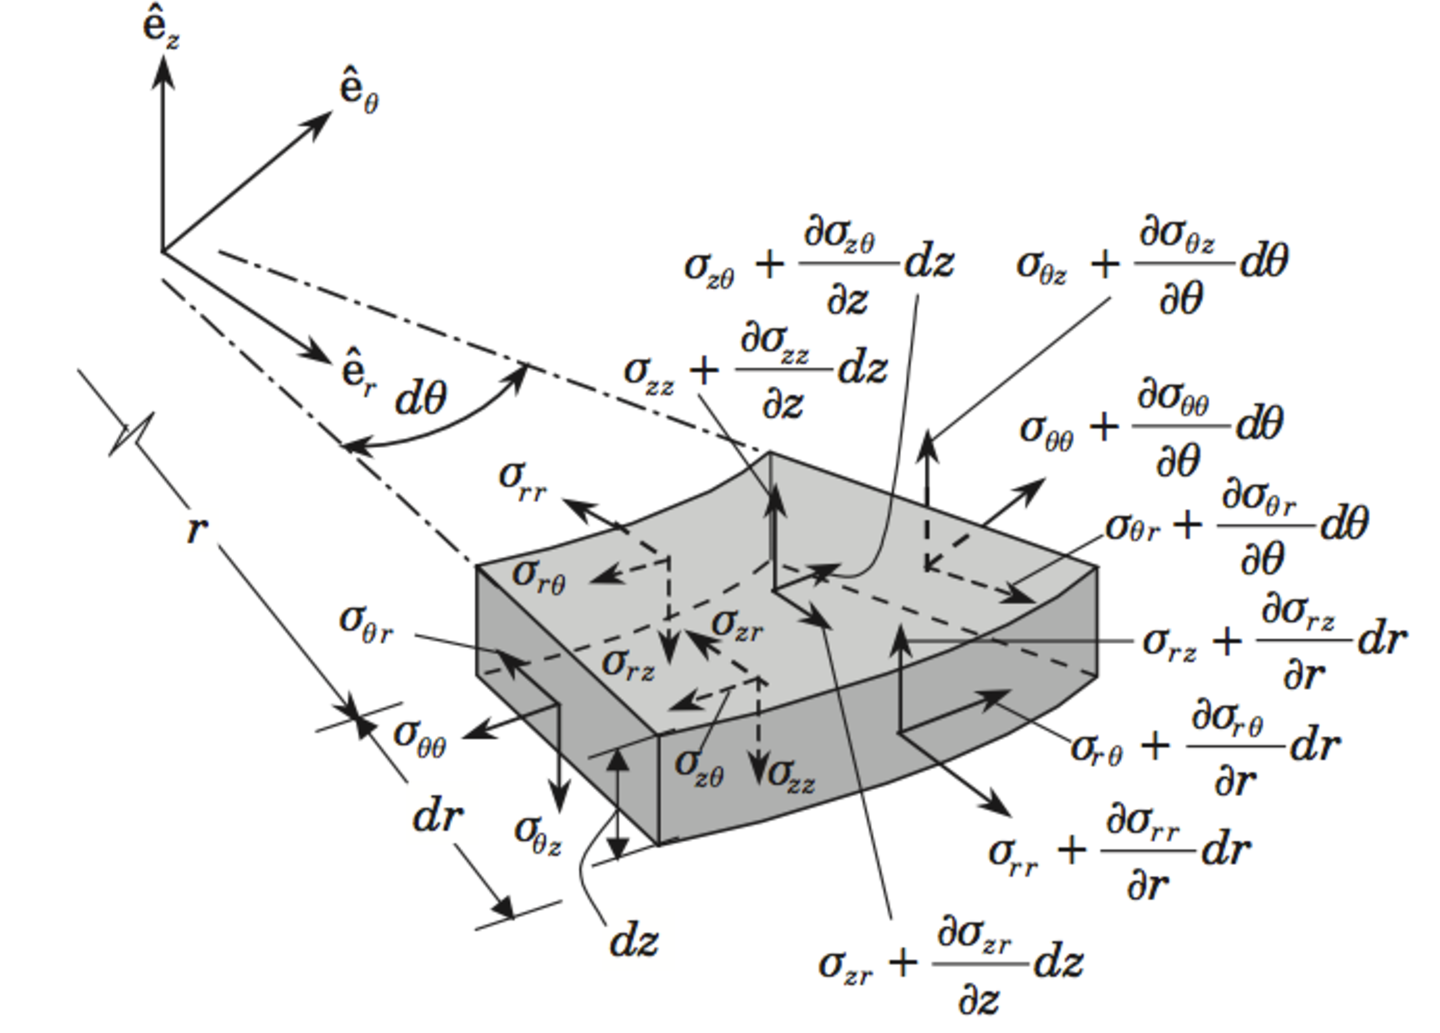
\includegraphics[width=4.0 in]{diffblockcil.pdf}
	\caption{Tensiones en un elemento diferencial de tamaño $dr{d\theta}dz$.}
	\label{diffcil}
\end{figure}

\begin{equation} \label{equcil}
\begin{split}
& \frac{{\partial {\sigma _{rr}}}}{{\partial r}} + \frac{1}{r}  \frac{{\partial {\tau _{{\theta}r}}}}{{\partial \theta}} + \frac{{\partial {\tau _{zr}}}}{{\partial z}} + \frac{\sigma _{rr} - \sigma _{{\theta}{\theta}}}{r} + {B_r} = 0 \\
& \frac{{\partial {\tau _{r{\theta}}}}}{{\partial r}} + \frac{1}{r} \frac{{\partial {\sigma _{{\theta}{\theta}}}}}{{\partial \theta}} + \frac{{\partial {\tau _{z{\theta}}}}}{{\partial z}} +  \frac{2 \tau_{r{\theta}}}{r} + {B_\theta} = 0 \\
& \frac{{\partial {\tau _{rz}}}}{{\partial r}} + \frac{1}{r} \frac{{\partial {\tau _{{\theta}z}}}}{{\partial \theta}} + \frac{{\partial {\sigma _{zz}}}}{{\partial z}} + \frac{ \tau_{rz}}{r} + {B_z} = 0 
\end{split}
\end{equation}

\subsection*{Ejemplo 1: Cuña autosoportada}

Considere la cuña doble de lado $\ell$ y ángulo interno $2 \phi$ mostrada en la \cref{WEDGE}. Se asume que esta se encuentra contenida en el plano $X-Y$, con condiciones de carga idealizables mediante un estado plano de tensiones (es decir 2D). La cuña se encuentra cargada por tracciones uniformes de intensidad $S$ aplicadas sobre sus 4 caras de tal manera que esta se encuentra auto-equilibrada. Determinar la solución al problema de valores en la frontera {\bf proponiendo una solución y verificando las condiciones de frontera}.
\begin{figure}[H]
\centering
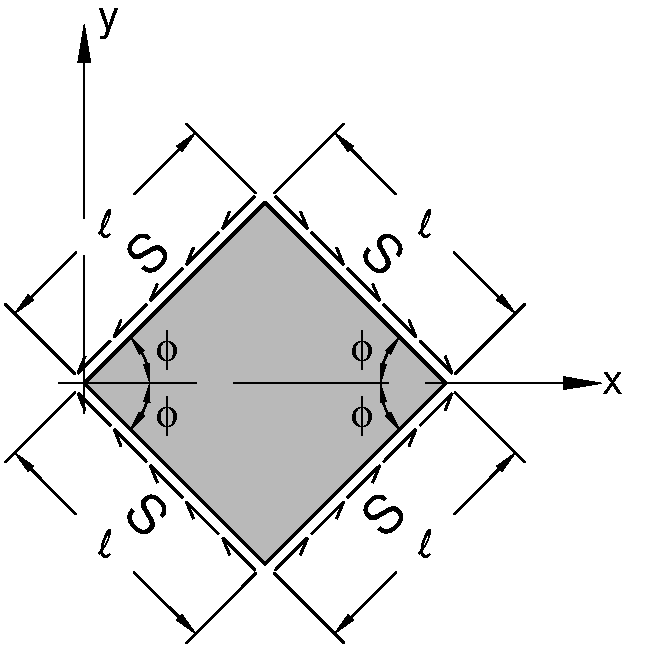
\includegraphics[width=8cm]{wedge.pdf}
\caption{2D Self-equilibrated wedge.}
\label{WEDGE}
\end{figure}


En el caso de estados de tensiones idealizables en 2 dimensiones y contenidos en el plano $x-y$ nada es función de $z$ y las ecuaciones de equlibrio \cref{equtr} y \cref{equrot} se reducen a
\begin{equation}
\begin{aligned}
&\dfrac{\partial\sigma_{xx}}{\partial x}+\dfrac{\partial\tau_{xy}}{\partial y}=0\\
&\dfrac{\partial\tau_{xy}}{\partial x}+\dfrac{\partial\sigma_{yy}}{\partial y}=0
\end{aligned}
\label{equilibrium}
\end{equation}

mientras que el equilibrio rotacional se reduce a
\[\tau_{xy} = \tau_{yx}.\]

Para proponer una solución planteamos las ecuaciones de equilibrio global de la cuña, lo cual es equivalente a asumir que las solución es constante. Se tiene entonces que
\begin{align*}
&\sum F_x=0 \longrightarrow -\ell S \cos\phi + \sigma_{xx}\ell \sin\phi=0\\
&\sum F_y=0 \longrightarrow -\ell S \sin\phi - \sigma_{yy}\ell \cos\phi=0
\end{align*}
de donde resulta la siguiente función para el campo de tensiones
\begin{equation}
\begin{aligned}
\sigma_{xx}&=S\cot\phi\\
\sigma_{yy}&=-S\tan\phi\\
\tau_{xy}&=0
\end{aligned}
\label{solution}
\end{equation}
con la condición $\tau_{xy}=0$ debida a la simetría del problema.

Para verificar que esta solución satisface las ecuaciones gobernantes reemplazamos la \cref{solution} en \cref{equilibrium}, notando que en este problema en particular no hay fuerzas de cuerpo ($\vec B = 0$)  resultando en;
\[\frac{\partial (S \cot\phi )}{\partial x} = 0\]
y
\[\frac{\partial (-S\tan\phi)}{\partial y} = 0.\]


Sin embargo, existen infinitas funciones $\sigma  = \sigma (x,y)$  que satisfacen las \cref{equilibrium} y para garantizar que la solución {\bf propuesta} es la solución correcta al problema es necesario verificar que esta satisface además las condiciones de frontera del problema.

Sean $\hat{n}^1$,$\hat{n}^2$,$\hat{n}^3$,$\hat{n}^4$ los vectores normales externos a las caras expuestas de la cuña y escritos en el sistema de referencia $x-y$ como;

\[\hat{n}^1 = -\sin\phi \hat{e}_{x} + \cos\phi \hat{e}_{y}\]
\[\hat{n}^2 = -\sin\phi \hat{e}_{x} - \cos\phi \hat{e}_{y}\]
\[\hat{n}^3 = +\sin\phi \hat{e}_{x} + \cos\phi \hat{e}_{y}\]
\[\hat{n}^4 = +\sin\phi \hat{e}_{x} - \cos\phi \hat{e}_{y}.\]


Para calcular las componentes del vector de tracciones sobre cada una de las caras usamos la fórmula de Cauchy escrita como
\[t_{i}=\sigma_{ij}\hat{n}_{j}.\]

Luego, sobre la cara con vector normal $\hat{n}^1$ tenemos
\begin{align*}
&t_{x}=-S \cos\phi\\
&t_{y}=-S \sin\phi\, ,
\end{align*}
similarmente sobre la cara con vector normal $\hat{n}^2$
\begin{align*}
&t_{x}=-S \cos\phi\\
&t_{y}=+S \sin\phi\, ,
\end{align*}
sobre la cara con vector normal $\hat{n}^3$
\begin{align*}
&t_{x} = +S \cos\phi\\
&t_{y} = -S \sin\phi\, ,
\end{align*}
y finalmente, sobre la cara con vector normal $\hat{n}^4$
\begin{align*}
&t_{x} = +S \cos\phi\\
&t_{y} = +S \sin\phi\, ,
\end{align*}
los cuales coinciden con las tracciones especificadas como condiciones de frontera del problema.


\subsection*{Ejemplo 2: Empujes sobre presa de concreto}

Si se sabe que la función de tensiones dada en la \cref{sln1} es solución al problema de valores en la frontera del medio continuo sobre el dominio mostrado en la \cref{dam}, en donde $\gamma$ es una constante.\footnote{Un script de Python con las funciones de esfuerzo está disponible en: \url{https://github.com/casierraa/MMC/blob/master/dam.py}.} Se pide:
\begin{equation}
\begin{split}
\sigma_{xx} & = \gamma x - 2\gamma y \\
\sigma_{yy} & =  - \gamma x \\
\tau_{xy}   & =  - \gamma y
\end{split}
\label{sln1}
\end{equation}

\begin{figure}[H]
\centering
	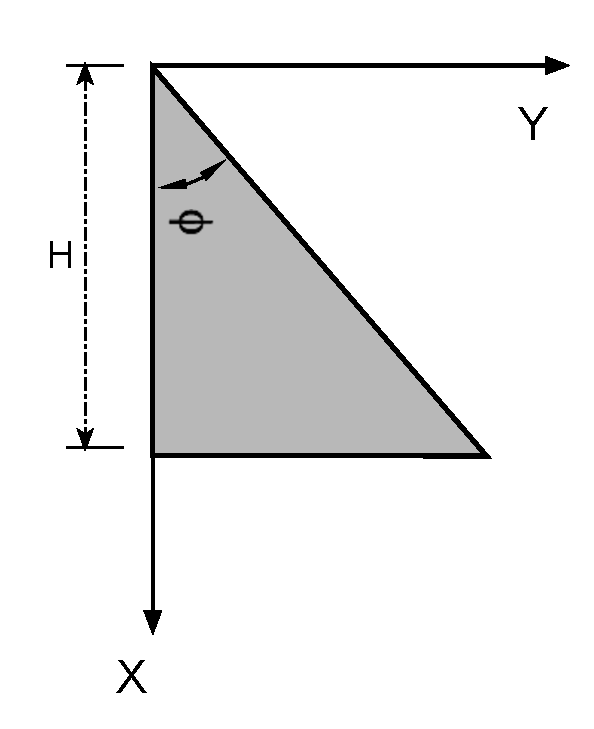
\includegraphics[width=2 in]{dam.pdf}
	\caption{Dominio de validez de la solución.}
	\label{dam}
\end{figure}


\begin{itemize}
\item[•] Identificar la frontera del problema.
\item[•] Verificar que la función dada en la \cref{sln1} efectivamente satisface las condiciones de equilibrio local.
\item[•] Determinar las condiciones de frontera sobre el dominio (graficar).
\item[•] Verificar que la solución satisface condiciones de equilibrio global.
\end{itemize}


\subsubsection*{Solución}
Sustituyendo la solución dada en \cref{sln1} en las ecuaciones de equilibrio local y considerando que $B_x =0$ y $B_y =0$ se verifica que la solución satisface equilibrio
\[\frac{{\partial (\gamma x - 2\gamma y)}}{{\partial x}} + \frac{{\partial ( - \gamma y)}}{{\partial y}} + {B_x} = 0\]
\[\gamma  - \gamma  = 0\] 
\[\frac{{\partial ( - \gamma y)}}{{\partial x}} + \frac{{\partial ( - \gamma x)}}{{\partial y}} + {B_y} = 0\]
\[0 + 0 = 0.\]

Sean los vectores normales a las caras vertical, horizontal e inclinada ${{\hat n}^1} =  - \hat j$, ${{\hat n}^2} =   \hat i$ y ${{\hat n}^3} =  - {S_\phi }\hat i + {C_\phi }\hat j$ respectivamente. En la superficie con normal ${{\hat n}^1}$ ($y=0$) se tiene que;
\[{\sigma _{xx}} = \gamma x\]
\[{\sigma _{yy}} =  - \gamma x\]
y
\[{\tau _{xy}} = 0 \]
luego
\[\left\{ {\begin{array}{*{20}{c}}
{{t_x}}\\
{{t_y}}
\end{array}} \right\} = \left[ {\begin{array}{*{20}{c}}
{\gamma x}&0\\
0&{ - \gamma x}
\end{array}} \right]\left\{ {\begin{array}{*{20}{c}}
0\\
{ - 1}
\end{array}} \right\} = \left\{ {\begin{array}{*{20}{c}}
0\\
{\gamma x}
\end{array}} \right\}\]
esta distribución se muestra en la \cref{sigy}

\begin{figure}[H]
\centering
	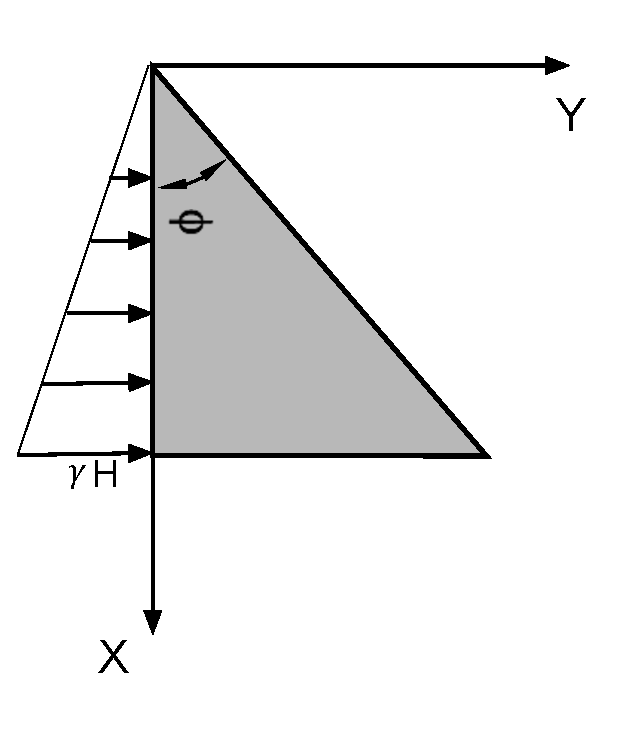
\includegraphics[width=2.0 in]{sigy.pdf}
	\caption{Distribución de tracciones sobre la cara vertical.}
	\label{sigx}
\end{figure}


Similarmente, sobre la superficie con normal $\hat{n}^2 =   \hat\imath$ ($x=H$) se tiene
\begin{align*}
&\sigma_{xx} = \gamma H - 2\gamma y\\
&\sigma_{yy} =  -\gamma H
\end{align*}
y
\[\tau_{xy} =  - gamma y\]
luego
\[\left\{ {\begin{array}{*{20}{c}}
{{t_x}}\\
{{t_y}}
\end{array}} \right\} = \left[ {\begin{array}{*{20}{c}}
{\gamma H - 2\gamma y}&{ - \gamma y}\\
{ - \gamma y}&{ - \gamma H}
\end{array}} \right]\left\{ {\begin{array}{*{20}{c}}
1\\
0
\end{array}} \right\} = \left\{ {\begin{array}{*{20}{c}}
{\gamma H - 2\gamma y}\\
{ - \gamma y}
\end{array}} \right\}.\]


La distribución de la componente $t_x$ sobre esta cara, corresponde a la tensión normal $\sigma_{xx}$ tal y como se muestra en la \cref{sigx}.
\begin{figure}[H]
\centering
	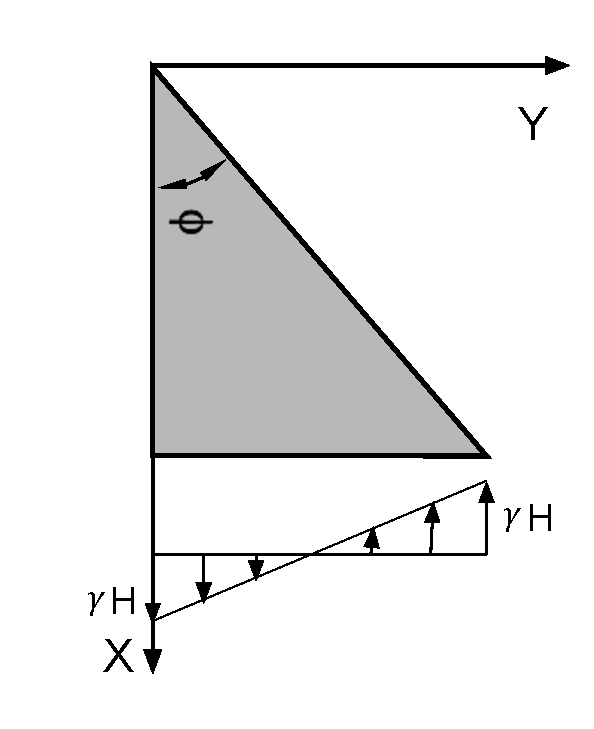
\includegraphics[width=2.0 in]{sigx.pdf}
	\caption{Distribución de tensiones normales sobre la cara horizontal.}
	\label{sigy}
\end{figure}

Similarmente, la componente $t_y$ corresponde a la componente $\tau_{xy}$. Sobre esta cara se tiene en $y=0$  que $t_y = 0$, mientras que en $y=H$ $t_y = - \gamma H$. Esta distribución se muestra en la \cref{taoxy}
\begin{figure}[H]
\centering
	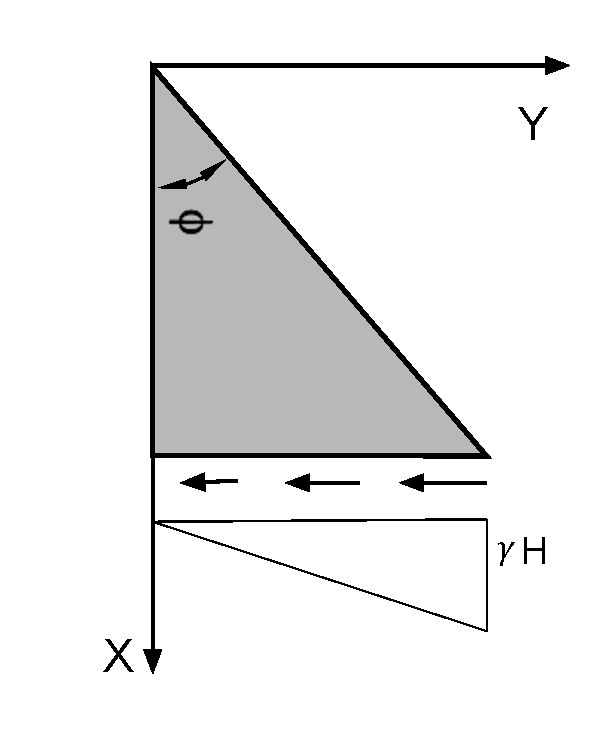
\includegraphics[width=2.0 in]{tauxy.pdf}
	\caption{Distribución de tensiones cortantes sobre la cara horizontal.}
	\label{taoxy}
\end{figure}


En la \cref{fig:contornos_presa} se presentan las distribuciones de tensiones sobre toda la presa en forma de contornos y curvas de nivel de isotensiones (igual valor de tensión).
\begin{figure}[H]
     \centering
     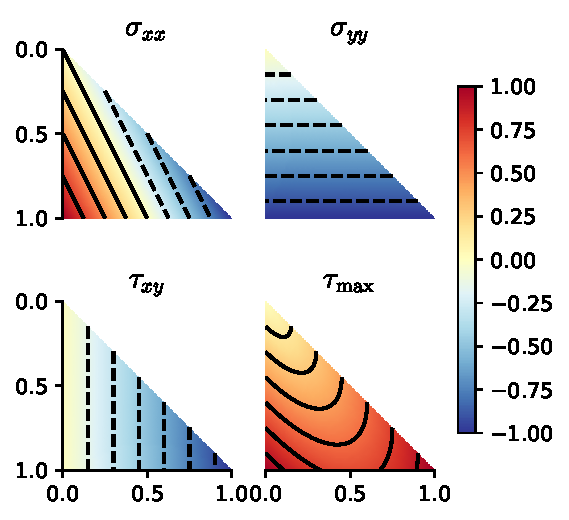
\includegraphics[width=3.5 in]{presa_esfuerzos.pdf}
     \caption{Variación de las tensiones que producen fuerzas en la dirección $x$ y $y$ sobre la presa.}
     \label{fig:contornos_presa}
\end{figure}


Para verificar el equilibrio global consideremos el diagrama de cuerpo libre mostrado en la \cref{dcl}
\begin{figure}[H]
\centering
	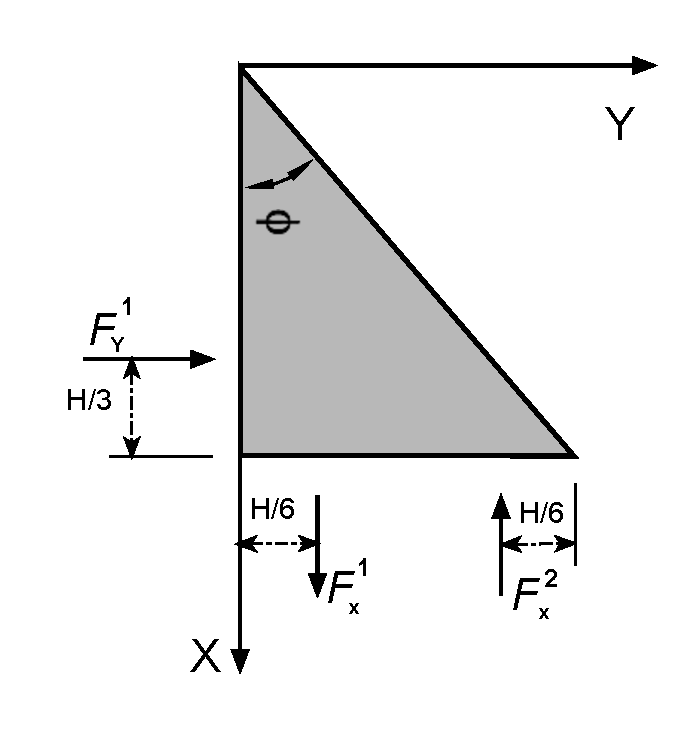
\includegraphics[width=2.0 in]{fbodydam.pdf}
	\caption{Diagrama de cuerpo libre de la presa.}
	\label{dcl}
\end{figure}
donde
\[F_x^1 = \frac{\gamma H^2}{4}\, ,\quad
F_x^2 =  - \frac{\gamma H^2}{4}\, ,\]
luego
\[\sum {{F_x} = 0} \]
y
\[F_y^1 = \frac{{\gamma {H^2}}}{2}\]
luego
\[\sum {{F_y} = 0} \]
similarmente
\[\sum {{M_A} = } \frac{4}{{24}}\gamma {H^3} + \frac{1}{{24}}\gamma {H^3} - \frac{5}{{24}}\gamma {H^3} = 0\]
con lo que se verifica que la solución satisface equilibrio global.

\subsection*{Tarea}
Para el problema de la presa;

\begin{itemize}
\item[•] Demostrar que la solución dada solo es valida para $\phi = \pi/4$
\item[•] Si la presa es de concreto, el cual presenta baja resistencia a la tracción determinar la zona de la presa que se debe reforzar para que esta no flalle. Nota: Identificar la superficie donde las tensiones normales ($\sigma_{xx}$) cambian de compresión a tracción.
\end{itemize}

\section{Soluciones clásicas para sólidos}
En esta sección se presentan algunas soluciones clásicas en términos de tensiones. Se inivta al estudiante a realizar el análisis de las mismas usando razonamientos similares a los presentados en los 2 ejemplos anteriores y de acuerdo con los objetivos de aprendizaje declarados al inicio del capitulo.

\subsection{Barra prismática soportada en la superficie superior y sometida a la acción de su propio peso}

La barra prismatica mostrada en la \cref{barra}

\begin{figure}[H]
\centering
	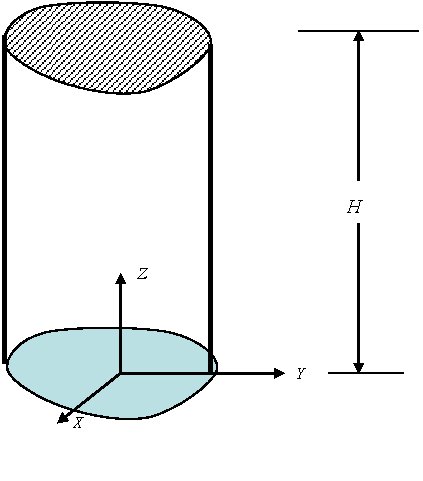
\includegraphics[width=2.5 in]{barrapp.pdf}
	\caption{Barra prismática sometica a la acción de peso propio.}
	\label{barra}
\end{figure}

se encuentra atada sobre la superficie superior y esta sometida a la acción de su propio peso. La función dada en la \cref{slnb} es la solución del problema,


\begin{equation}
\begin{split}
{\sigma _{zz}} & = \gamma z \\
{\sigma _{xx}} & = {\sigma _{yy}} = 0 \\
{\tau _{xy}}   & = {\tau _{xz}} = {\tau _{yz}} = 0
\end{split}
\label{slnb}
\end{equation}


\subsection{Viga en voladizo}

La \cref{Viga} muestra una viga en voladizo sometida a una carga $P$ en uno de sus extremos: 
\begin{figure}[H]
\centering
	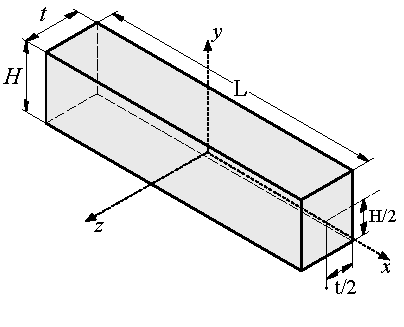
\includegraphics[width=3.0 in]{Viga.pdf}
	\caption{Viga en voladizo.}
	\label{Viga}
\end{figure}

El tensor solución se da en la \cref{slnc}.
\begin{equation}
\begin{split}
{\sigma_{xx}} & = - \dfrac{P}{I} (XY) \\
 {\sigma_{yy} }&= \sigma_{zz} = 0 \\
{\tau_{xy}} & = \tau_{yx} = - \dfrac{P}{2I} (\dfrac{H^2}{4} - Y^2) \\ 
{\tau_{xz}} &= 0
\end{split}	
\label{viga}
\end{equation}


\subsection{Cilindro sometido a presión interna y externa}
Para este problema se requieren las ecuaciones de equilibrio local en coordenadas polares dadas por:
\begin{equation} \label{equcil}
\begin{split}
& \frac{{\partial {\sigma _{rr}}}}{{\partial r}} + \frac{1}{r}\frac{{\partial {\tau _{\theta r}}}}{{\partial \theta }} + \frac{{{\sigma _{rr}} - {\sigma _{\theta \theta }}}}{r} + {B_r} = 0 \\
& \frac{{\partial {\tau _{\theta r}}}}{{\partial r}} + \frac{1}{r}\frac{{\partial {\sigma _{\theta \theta }}}}{{\partial \theta }} + \frac{{2{\tau _{r\theta }}}}{r} + {B_\theta } = 0
\end{split}
\end{equation}

La \cref{cilindro} muestra un cilindro de radio interno $a$ y radio externo $b$ sometido a presiones internas y externas $p_a$ y $p_b$ respectivamente
\begin{figure}[H]
\centering
	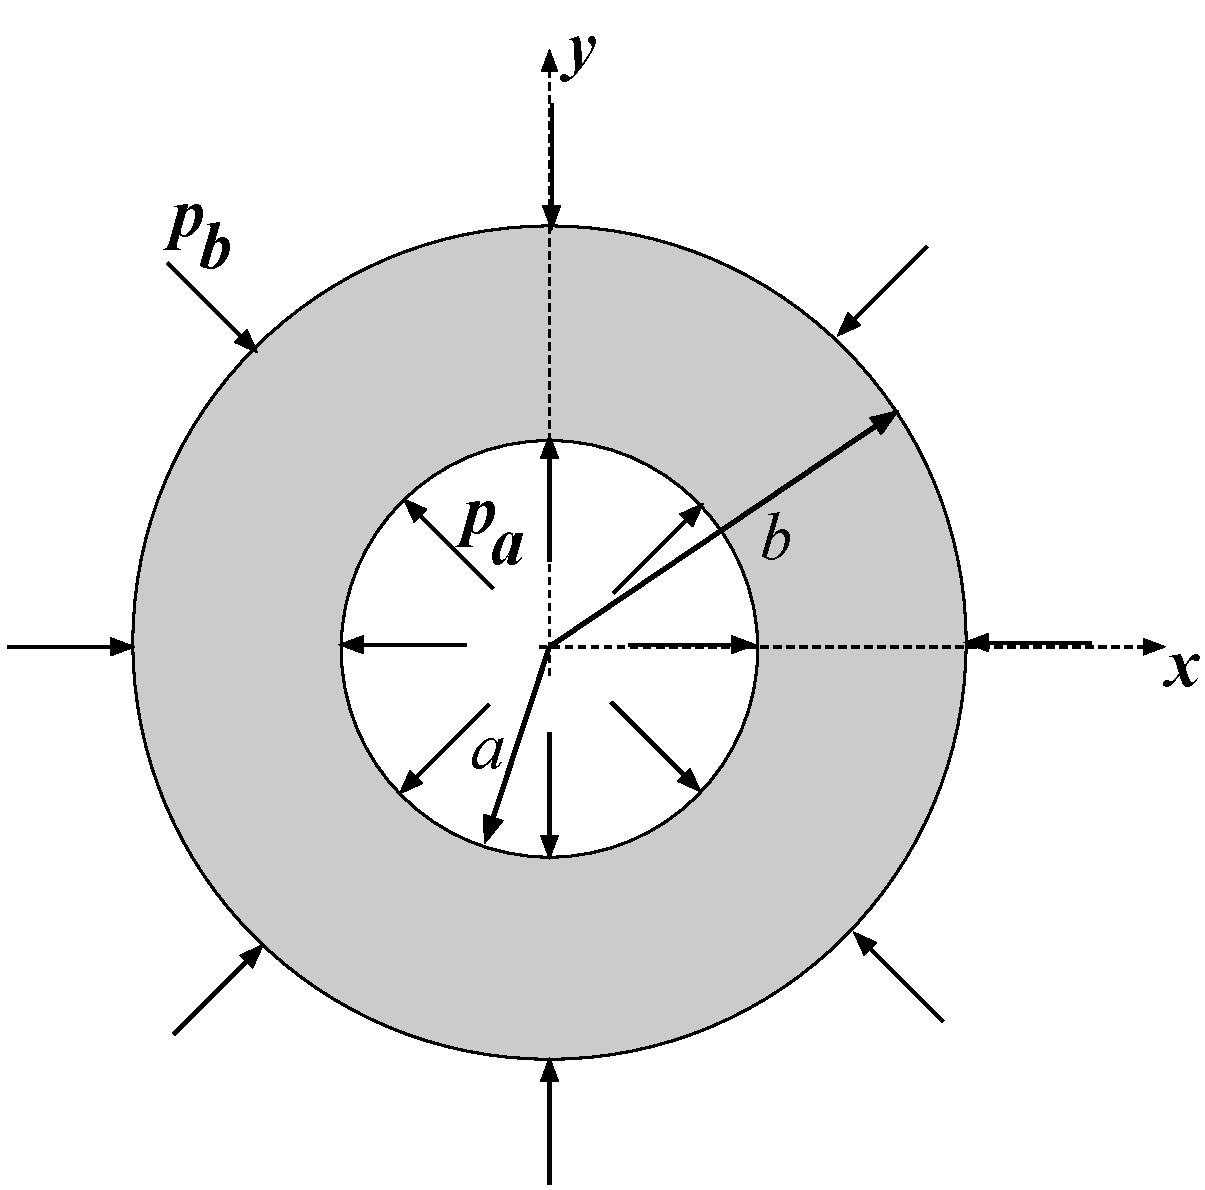
\includegraphics[width=3.0 in]{cilindro.pdf}
	\caption{Cilindro sometido a presión interna y externa.}
	\label{cilindro}
\end{figure}

El tensor solución se da en la \cref{slnc}\begin{equation}
\begin{split}
\sigma_{rr} & =  - \frac{\left( \frac{b^2}{r^2} - 1 \right)}{\left(\frac{b^2}{a^2} - 1\right)} p_a - \frac{\left(1 - \frac{a^2}{r^2} \right)} {\left(1 - \frac{a^2}{b^2} \right)} p_b \\
\sigma_{\theta\theta} & = \frac{\left(\frac{b^2}{r^2} + 1\right)}{\left(\frac{b^2}{a^2} - 1\right)} p_a - \frac{\left(1 + \frac{a^2}{r^2} \right)}{\left( 1 - \frac{a^2}{b^2}\right)} p_b
\end{split}
\label{slnc}
\end{equation}

\subsection{Flamant}
La \cref{Flamant} muestra un semi-espacio sometido a una carga lineal superficial \(P\). 

\begin{figure}[H]
\centering
	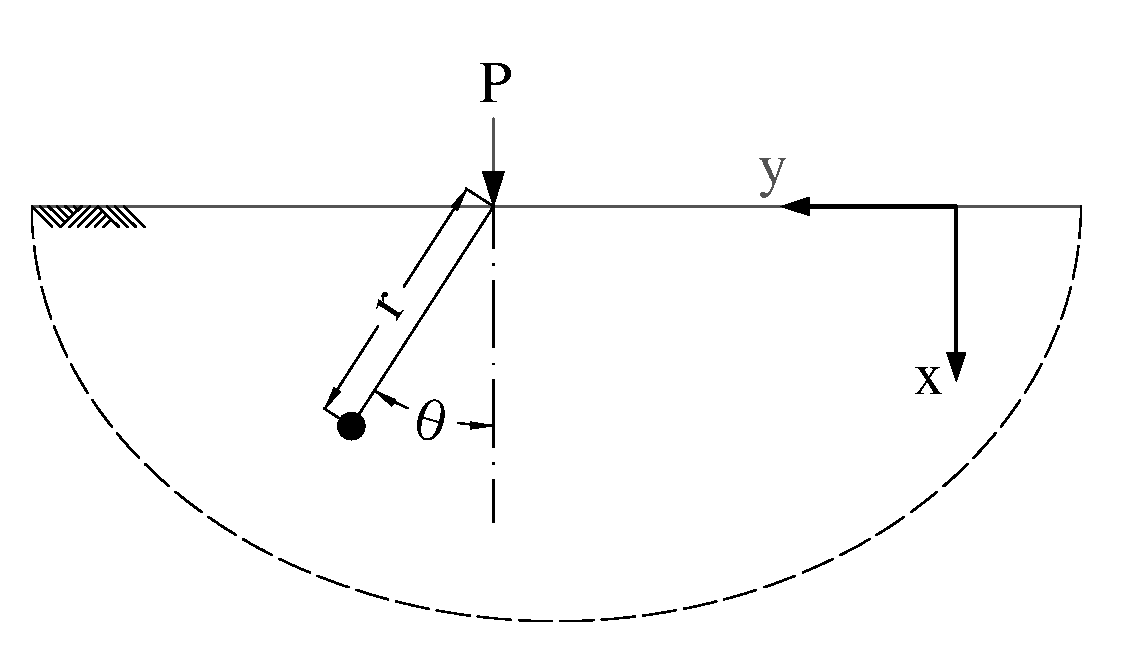
\includegraphics[width=3.0 in]{Bousinesq.pdf}
	\caption{Medio continuo sometido a una carga P.}
	\label{Flamant}
\end{figure}

El tensor solución se da en la \cref{slnf}

\begin{equation}
\begin{split}
{ \sigma_{rr}} & = -\dfrac{2P}{\pi r} Cos \theta \\
{\sigma_{\theta\theta}}  &= 0\\
{\tau_{r\theta}}&= 0
\end{split}
\label{slnf}
\end{equation}

\subsection*{Ejemplo 3: aplicación de solución para cilindro sometido a presión interna y externa}

\begin{enumerate} 

\item La solución para un cilindro de radio interno $a$ y radio externo $b$ sometido a presiones internas y externas $p_a$ y $p_b$ respectivamente (ver \cref{cilindro}), está dado por:

\begin{equation*}
\sigma _{rr}  =  - \frac{{\left( {\frac{{{b^2}}}{{{r^2}}} - 1} \right)}}{{\left( {\frac{{{b^2}}}{{{a^2}}} - 1} \right)}}{p_a} - \frac{{\left( {1 - \frac{{{a^2}}}{{{r^2}}}} \right)}}{{\left( {1 - \frac{{{a^2}}}{{{b^2}}}} \right)}}{p_b} \hspace{1.5cm}
\sigma _{\theta \theta } = \frac{{\left( {\frac{{{b^2}}}{{{r^2}}} + 1} \right)}}{{\left( {\frac{{{b^2}}}{{{a^2}}} - 1} \right)}}{p_a} - \frac{{\left( {1 + \frac{{{a^2}}}{{{r^2}}}} \right)}}{{\left( {1 - \frac{{{a^2}}}{{{b^2}}}} \right)}}{p_b} \hspace{1.5cm}
\tau _{r\theta} = 0
\label{slnc}
\end{equation*}

\begin{figure}[H]
\centering
	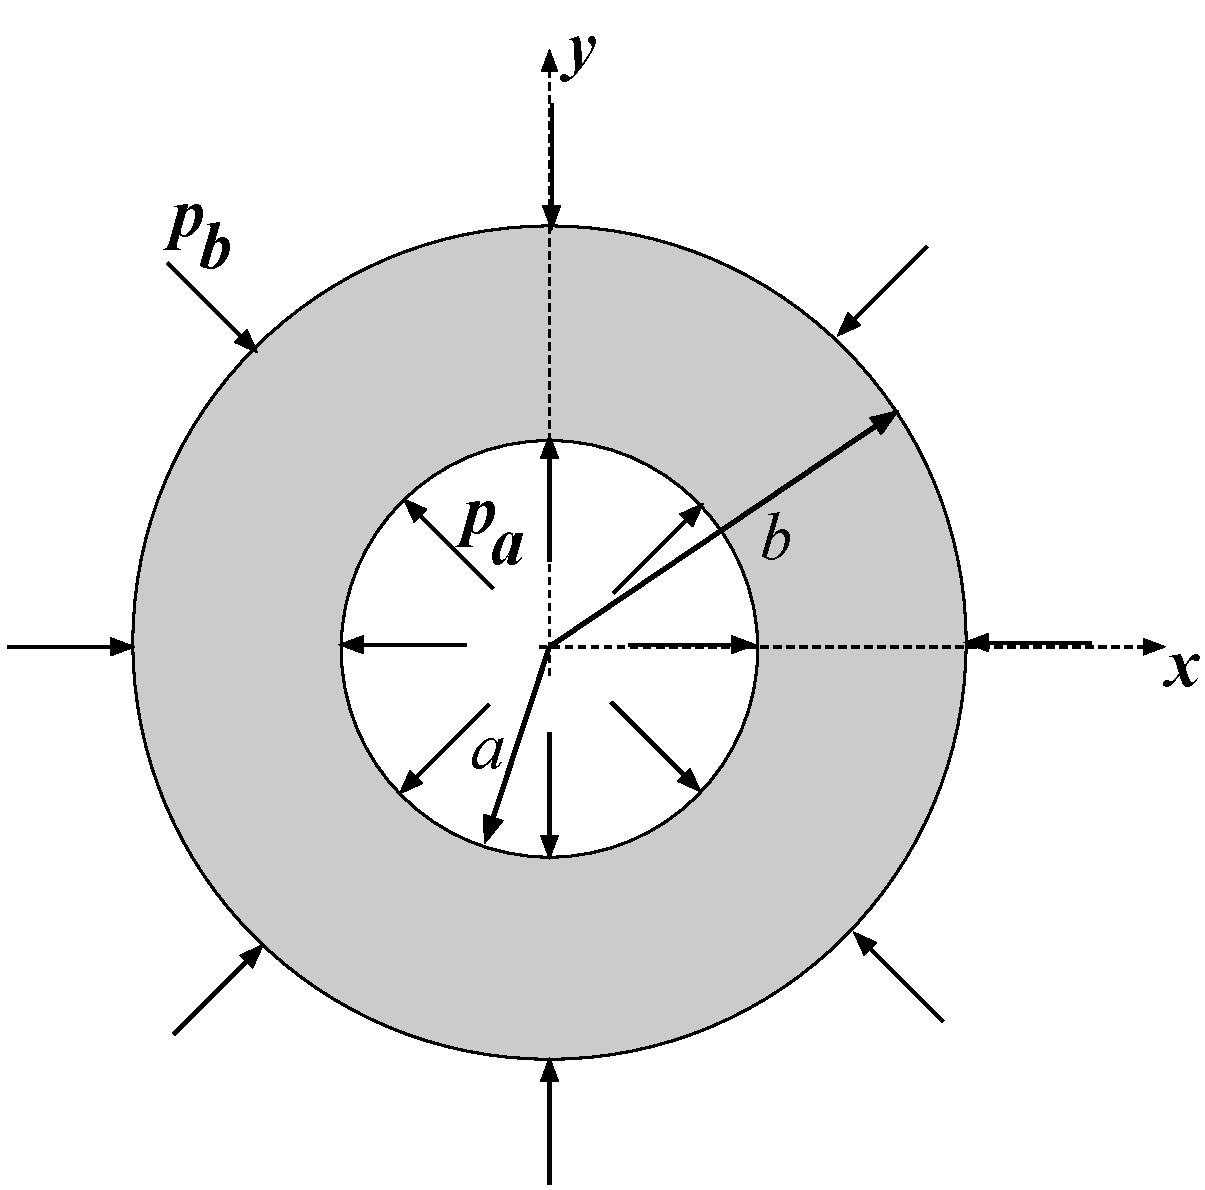
\includegraphics[width=3.0 in]{cilindro.pdf}
	\caption{Cilindro sometido a presión interna $p_a$ y presión externa $p_b$}
	\label{cilindro}
\end{figure}

\end{enumerate}

\subsection*{Ejemplo 4: Aplicación de soluciones}
En el enlace

\begin{enumerate} 
\item \small{\url{http://nbviewer.ipython.org/github/casierraa/Notebooks_MMC/blob/master/Ej5_Parcial2015.ipynb}}
\end{enumerate}

\newpage
\section{Ejercicios}

%\graphicspath{{imgTen/}} 	% Specifies the directory where pictures are

\begin{enumerate}
  
\item \label{punto01} Si el tensor de esfuerzos en cualquier punto de la cu\~na
presentada en la \cref{figure4} es:\\
	\\
	%
	$[\sigma] = \left[ \begin{array}{ccc}
	-S cot \phi & 0 \\ 
	0 & S tan \phi
	\end{array}  \right] $\\
	%
	\begin{figure}[H]
		\centering
		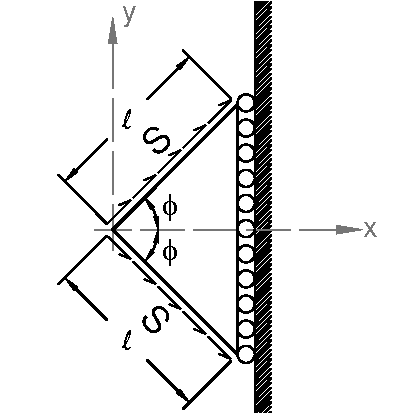
\includegraphics[height=6.25cm]{Ejer4_1.pdf}
		\caption{Cuña de espesor $e$ sometida a tensiones tangenciales constantes $(S)$ en dos caras.}
		\label{figure4}
	\end{figure}
	%
	\begin{enumerate}
		\item Verificar el equilibrio global $\left( \sum F = 0.0 \right)$.
		\item Verificar el equilibrio a nivel diferencial.
		\item  \textquestiondown Es posible encontrar esfuerzos cortantes $\tau_{xy}$ al interior de la cu\~na mayores a $S$?. Responder s\'i o no y justificar su respuesta.
		\item Calcule el vector de tensiones en cada cara de la cu\~na. 
	\end{enumerate}

\item \label{punto02} Encontrar las tensiones normales máximas y las direcciones
principales de un estado tensional que est\'a dado por el tensor de tensiones siguiente:
%
\[ [\sigma] = \left[ \begin{array}{ccc}
	1 & 1 & 0 \\ 
	1 & 4 & 0 \\ 
	0 & 0 & 2
\end{array}  \right]\]

\item \label{punto03}  En la \cref{barra:colga1} se muestra un elemento
con densidad $\rho$, de secci\'on circular, soportado de su extremo superior y est\'a sometido solamente a la acci\'on de su peso propio. Se indica el tensor de esfuerzos en el sistema coordenado $x-y$ para los puntos a y b mostrados en la figura.\\
	%
	\\
	Punto a: $[\sigma] = \left[ \begin{array}{ccc}
	0 & 0\\ 
	0 & 2 \gamma L/3\\
	\end{array}  \right] $
	\hspace{30mm}
	Punto b: $[\sigma] = \left[ \begin{array}{ccc}
	0 & 0\\ 
	0 & \gamma L/3\\
	\end{array}  \right] $ \\\\
	%
	\begin{figure}[H]
		\centering
		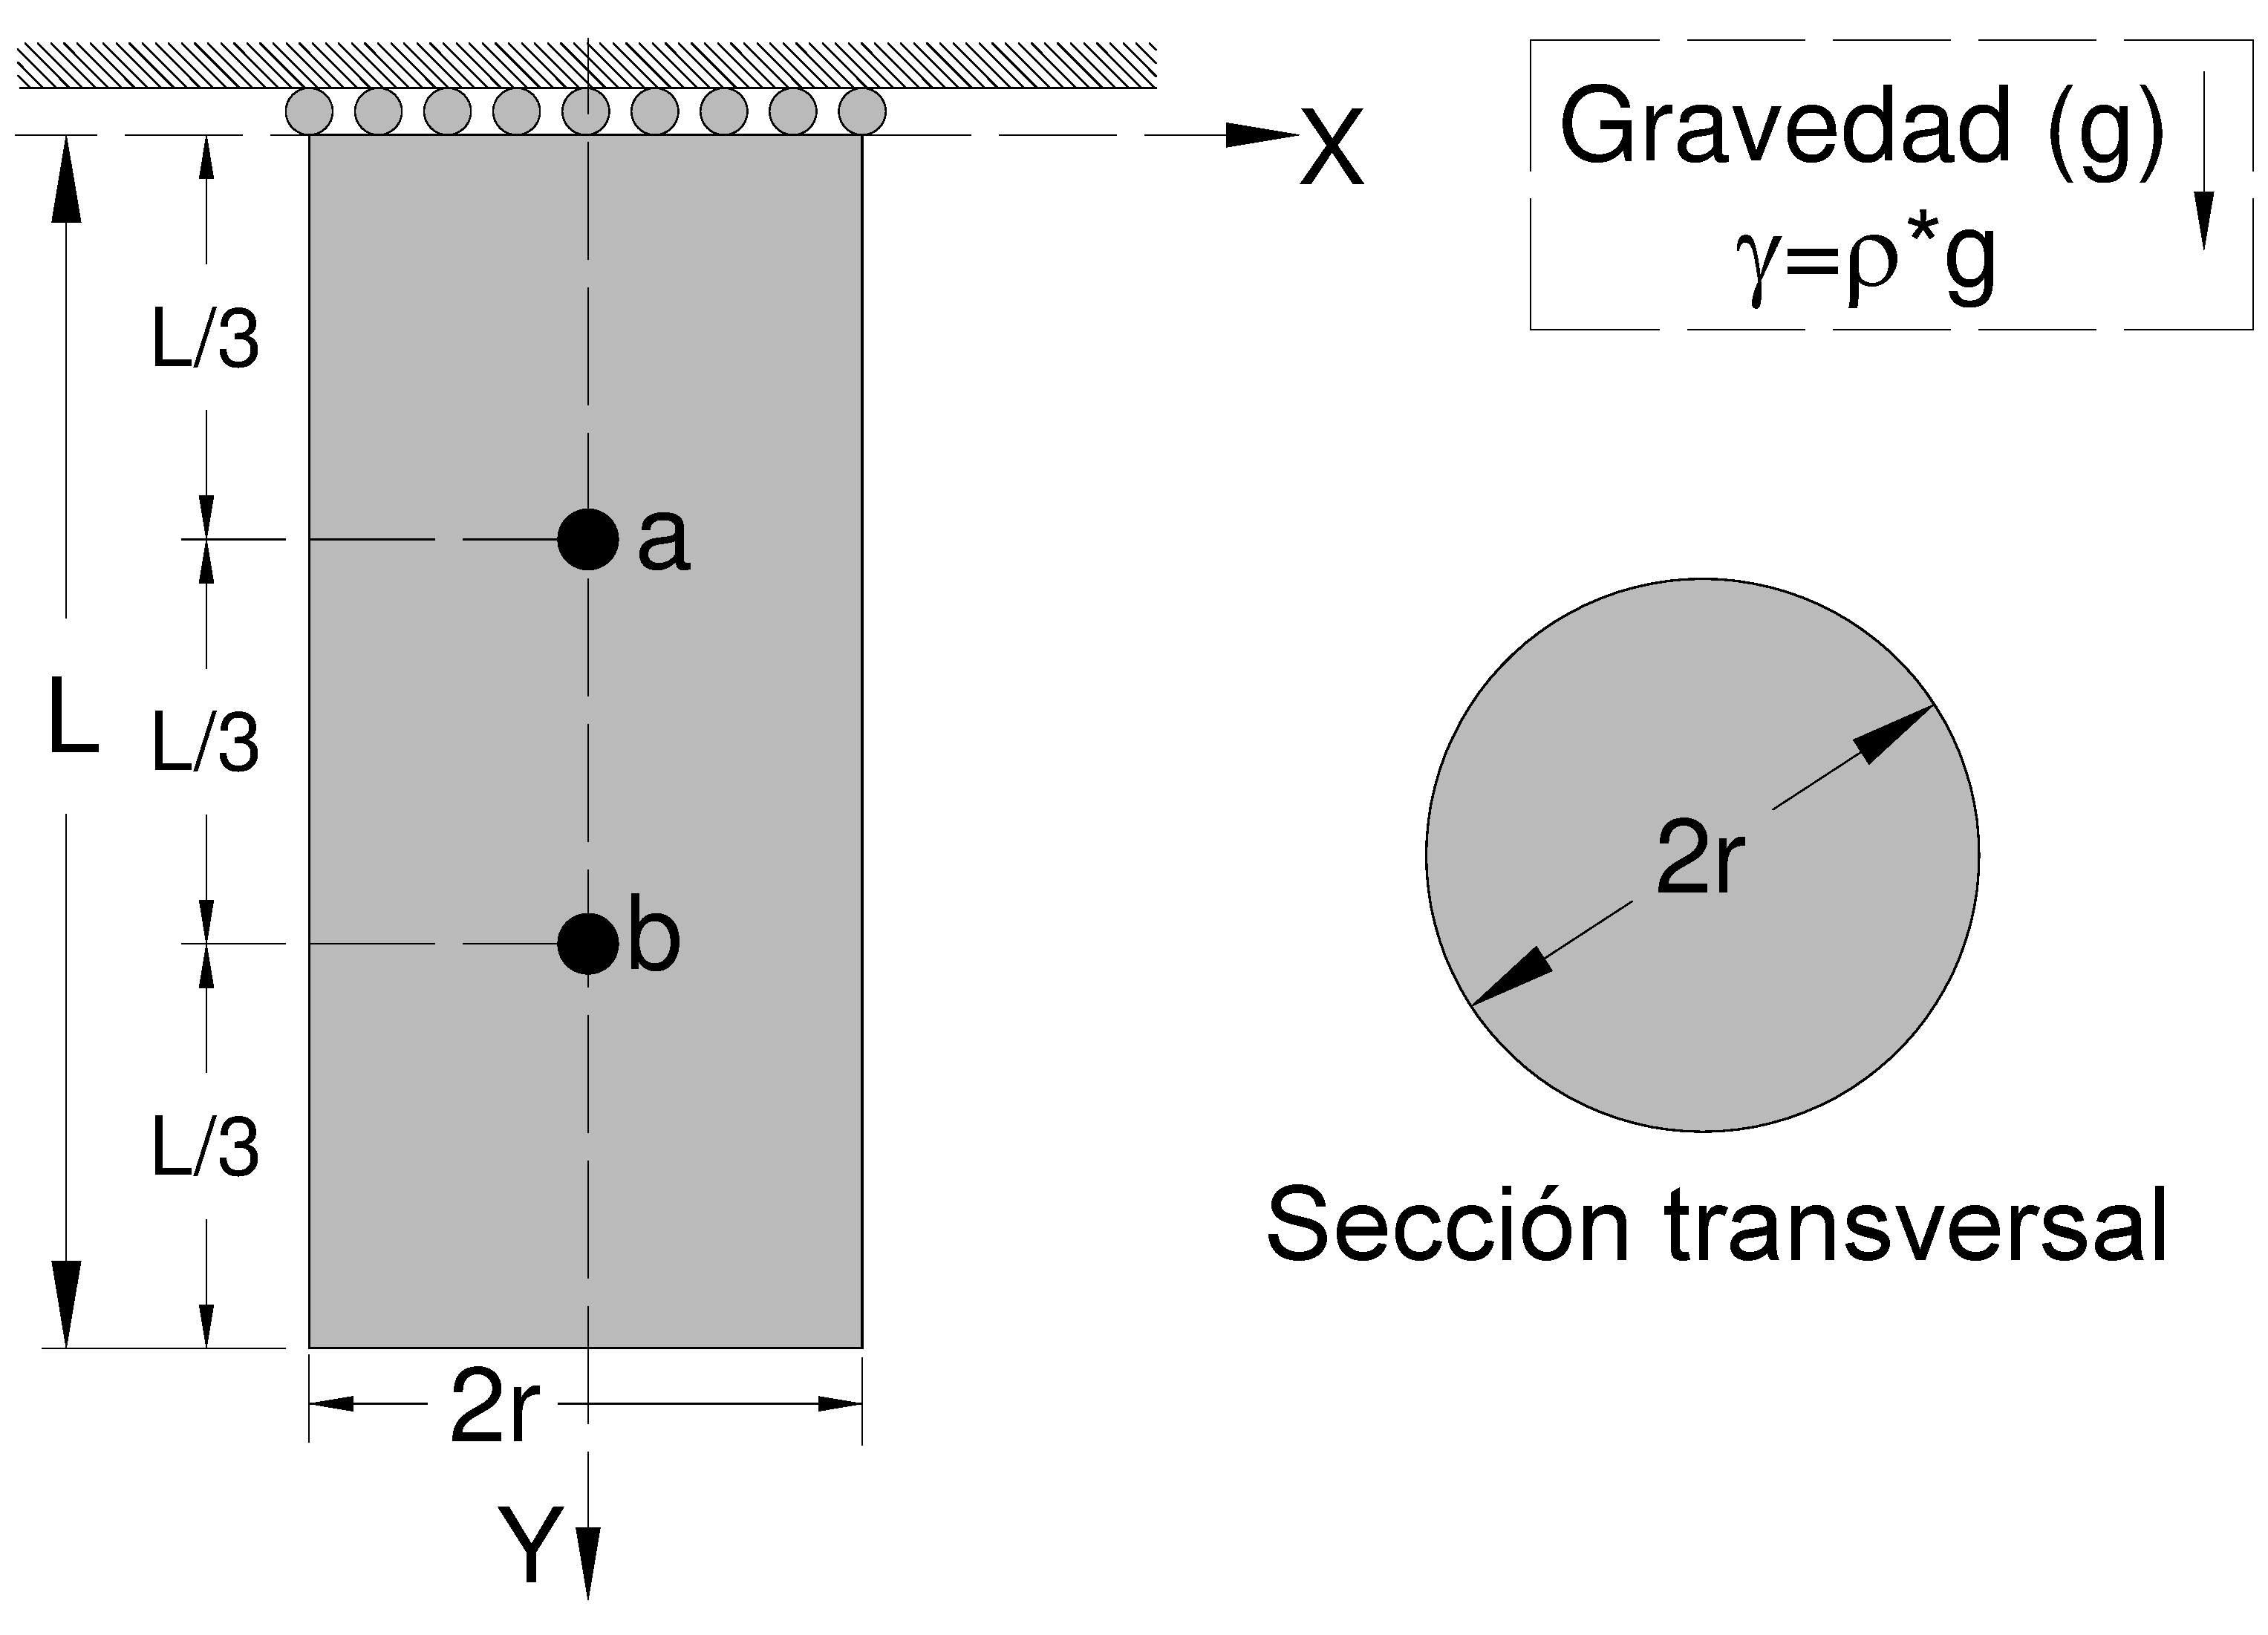
\includegraphics[height=5.75cm]{Ejer4_3.pdf}
		\caption{Barra colgada}
		 \label{barra:colga1}
	\end{figure}
	%
	Si el tensor de esfuerzos var\'ia de forma lineal a lo largo del eje $y$, se pide:
	%
	\begin{enumerate}
	% 
		\item El  tensor de esfuerzos para cualquier punto al interior del elemento. 
		\item \textquestiondown El elemento se encuentra en equilibrio a nivel diferencial?. Justifique su respuesta matem\'aticamente.
		\item Si el elemento es infinitamente resistente ante esfuerzos de tracci\'on y de compresi\'on, pero su capacidad m\'axima ante esfuerzos cortantes est\'a dada por \begin{large} $\tau_{max}$ \end{large}. Determine:
	%
		\begin{enumerate} 
			\item \textquestiondown Cu\'al es la longitud m\'axima posible del elemento?. 
			\item  \textquestiondown Cu\'al es la fuerza en el soporte superior cuando se produce la falla por corte?.
			\item \textquestiondown Cu\'al es la tensi\'on en la secci\'on transversal inferior del elemento  $\left( y=L \right)$  cuando se produce la falla por corte?.
		\end{enumerate}
%
		\item 	Si el elemento es infinitamente resistente ante esfuerzos cortantes y de compresi\'on, pero su capacidad m\'axima ante esfuerzos de tracci\'on est\'a dada por \begin{large} $\sigma_{trac}$ \end{large}. Determine:
		\begin{enumerate} 
			\item \textquestiondown Cu\'al es la longitud m\'axima posible del elemento?. 
			\item \textquestiondown Cu\'al es la tensi\'on en la secci\'on transversal inferior del elemento  $\left( y=L \right)$  cuando se produce la falla por tracci\'on?. 
			\item \textquestiondown Cu\'al es la fuerza en el soporte superior cuando se produce la falla por tracci\'on?.
		\end{enumerate}	
	
		\item	Si el elemento es infinitamente resistente ante esfuerzos cortantes y de tracci\'on, pero su capacidad m\'axima ante esfuerzos de compresi\'on est\'a dada por \begin{large} $\sigma_{comp}$ \end{large}. Determine: 
		\begin{enumerate}		
			\item \textquestiondown Cu\'al es la longitud m\'axima posible del elemento?. 
			\item \textquestiondown Cu\'al es la tensi\'on en la secci\'on transversal inferior del elemento  $\left( y=L \right)$  cuando se produce la falla por compresi\'on?. 
			\item \textquestiondown Cu\'al es la fuerza en el soporte superior cuando se produce la falla por compresi\'on?.
		\end{enumerate}
	\end{enumerate}


\item \label{punto04} El tensor de tensiones de un medio continuo se describe
con la siguiente di\'adica:
		\[ [\sigma] = \left[ \begin{array}{ccc}
		-2x^2yx & 4z^2+yx & 2z^2yx-xz \\ 
		4z^2+yx & yz+4y^2 & -yz-xyz \\ 
		2z^2yx-xz & -yz-xyz & 4z^3
		\end{array}  \right] \enspace\]
		%
	\begin{enumerate}
		\item Calcular la fuerza de cuerpo necesaria para mantener el medio continuo en equilibrio est\'atico.
%		\item Calcular la fuerza de cuerpo necesaria para mantener el medio continuo en equilibrio din\'amico si se tiene el campo de velocidades $v_x=xt$, $v_y=xy$ y $v_z=zt$.
	\end{enumerate}
% *************************** %
\item \label{punto05} Si en un medio continuo, el campo de tensiones est\'a dado
por el tensor:
		\[ [\sigma] = \left[ \begin{array}{ccc}
		x^2y & (1-y^2)x & 0 \\ 
		(1-y^2)x & (y^3-3y)/3 & 0 \\ 
		0 & 0 & 2z^2
		\end{array}  \right]\enspace \]
		%
	Determinar:
	%
	\begin{enumerate}
		\item La fuerza de cuerpo necesaria para mantener el medio continuo en equilibrio est\'atico.
		\item Las tensiones principales en el punto $P(a,0,0)$.
		\item La tensi\'on tangencial (corte) m\'axima en el punto $P$.
%		\item Las fuerzas de cuerpo necesarias para que se cumpla el equilibrio din\'amico si se tiene el campo de velocidades $v_x=xy$, $v_y=x^2t$ y $v_z=xyzt$.
	\end{enumerate}
% *************************** %
\item  \label{punto06} El campo de tensi\'on de un medio continuo está dado por: \footnote{Tomado del problema 4.4 en Reddy, J.N (2010). An introduction to continuum mechanics}
		\[[\sigma] = \left[ \begin{array}{ccc}
		0 & 0 & 2x_2 \\ 
		0 & 1 & 4x_1 \\ 
		2x_2 & 4x_1 & 1
		\end{array}  \right] \]
		%
	donde $x_1$ y $x_2$ son coordenadas cartesianas.

	\begin{enumerate}
		\item Despreciando las fuerzas de cuerpo \textquestiondown est\'a el cuerpo en equilibrio?
		\item Determinar el vector tensi\'on que act\'ua en un punto $(1,2,3)$ seg\'un el plano $x_1+x_2+x_3=6$;
		\item Determinar la proyecci\'on del vector tensi\'on seg\'un la direcci\'on normal y tangencial al plano $x_1 +x_2 +x_3 = 6$.
	\end{enumerate}
% *************************** %


\item \label{punto07} El campo del tensor de tensiones de Cauchy viene
representado por sus componentes como:
		\[[\sigma] = k\left[ \begin{array}{ccc}
		x_1^2 x_2 & (a^2-x_2^2)x_1 & 0 \\ 
		(a^2-x_2^2)x_1 & \frac{1}{3}(x_2^3 - 3a^2 x_2) & 0 \\ 
		0 & 0 & 2ax_3^2
		\end{array}  \right] \enspace,\]
%	
	donde $k$ y $a$ son constantes.
%
	Encontrar el campo de fuerzas de cuerpo $\mathbf{b}$ (por unidad de volumen) necesario para que el sistema est\'e en equilibrio.
%
\item \label{punto11} En la \cref{solucion} se muestra la solución fundamental para semi-espacio
sometido a una carga lineal superficial, $P$. Los esfuerzos al interior del suelo est\'an dados por: \\

		$\sigma_{xx}= -\dfrac{2P}{\pi r} Cos^3 \theta$ \hspace{10mm}
		$\sigma_{yy}= -\dfrac{2P}{\pi r} Sen^2 \theta Cos \theta $ \hspace{10mm}
		$\tau_{xy}= -\dfrac{2P}{\pi r} Sen \theta Cos^2 \theta $ \\\\
	%
\begin{figure}[H]
	\centering
		\subfloat [Solución fundamental carga superficial]{ 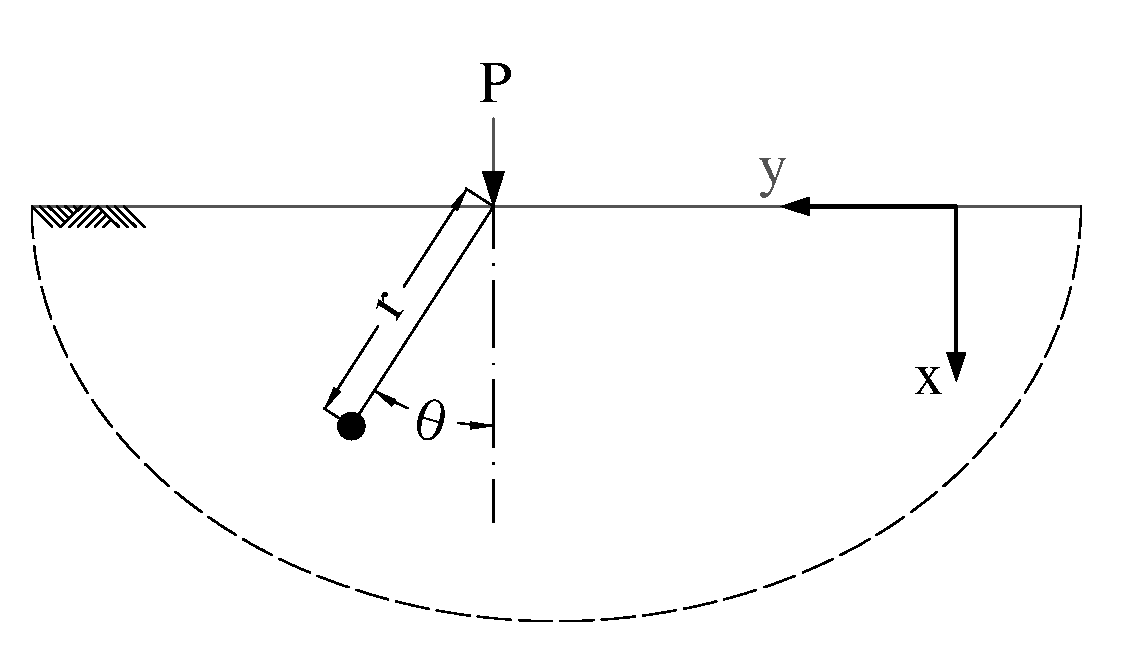
\includegraphics[width=2.7in]{Ejer4_11_1.pdf}\label{solucion}}
		\hspace{0.5cm}
		\subfloat [Estructuras y tuber\'ia. $L1 = 6 m$, $L2 = 10 m$, $H = 12 m$]{ 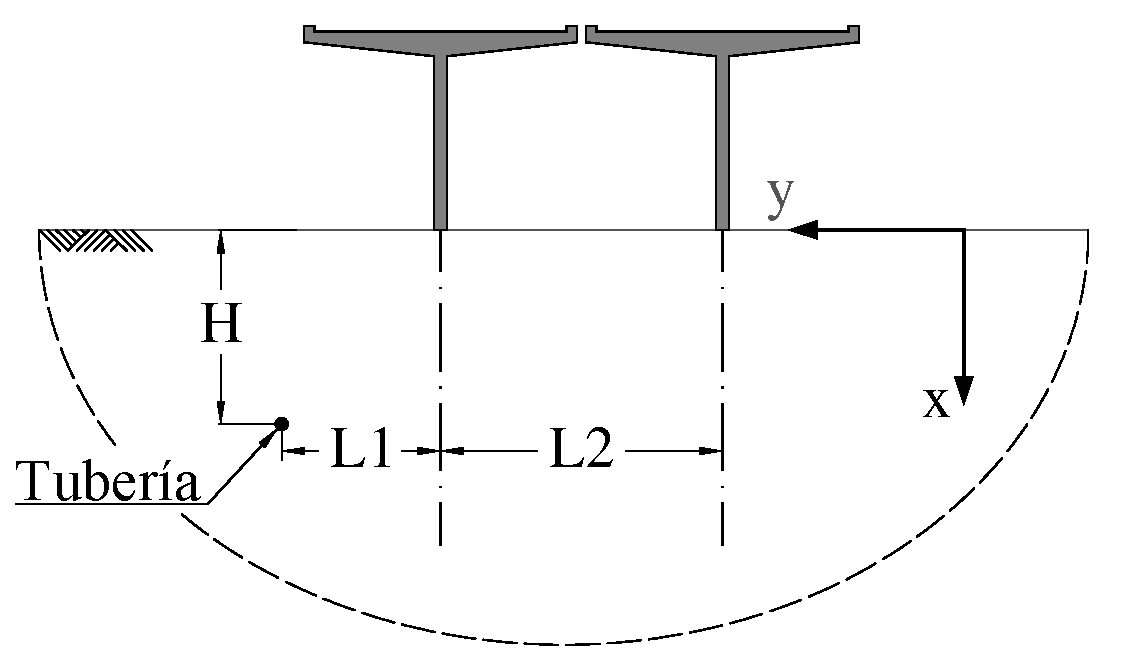
\includegraphics[width=2.6in]{Ejer4_11_2.pdf}\label{tuberia}}		
	\caption{Estructuras sobre la superficie}
	\label{figure1} 
\end{figure}
	%
S\'i se desea instalar una tuber\'ia, perpendicular al plano mostrado ($XY$), de d\'iametro despreciable en el punto indicado  en la \cref{tuberia}, y se sabe que el suelo  está sometido a la acción de dos estructuras que le transmiten de forma independiente una carga lineal superficial, $P=100$ $Ton/m $.  Determine:
	%
	\begin{enumerate}
	% 
		\item \textquestiondown Cu\'al es el esfuerzo m\'inimo de compresi\'on que debe ser capaz de soportar la tuber\'ia para que no se da\~ne?.
		\item \textquestiondown Cu\'al es el esfuerzo m\'inimo de cortante que debe ser capaz de soportar la tuber\'ia para que no se da\~ne?.
	\end{enumerate}
%
\item \label{punto12} El campo de tensi\'on de un medio continuo está
representado por: \\

	\begin{large}
		$[\sigma] = \left[ \begin{array}{ccc}
		a & a & a \\ 
		a & a & a \\
		a & a & a
		\end{array}  \right] $ \\
	\end{large}

	donde $a$ es una constante.

	\begin{enumerate}
		\item Determinar los valores principales.
		\item Determinar las direcciones principales.
		\item Determinar el valor del esfuerzo cortante máximo.
	\end{enumerate}
	%
\item \label{punto13} En la figura \ref{continuo} se muestra un cuerpo cuyo
tensor de esfuerzos  $[\sigma]$  en el sistema de referencia $xy$ est\'a dado  por:\\\\
	%
	$\sigma_{xx} = \dfrac{q}{8c^3} (2x^3y - 4xy^3 + \dfrac{12}{5}c^2xy) - px$ \hspace{30mm} $\sigma_{yy} = - \dfrac{q}{8c^3} (4c^3x - 2xy^3 + 6c^2xy)$ \\\\
	$\tau_{xy} = \tau_{yx} = \dfrac{q}{8c^3} [3x^2(c^2 - y^2)- (c^4 - y^4) + \dfrac{6}{5}c^2(c^2 - y^2)] $\\\\
	%
	Donde $q$, $p$ y $c$ son constantes.
	%
	\begin{figure}[H]
		\centering
		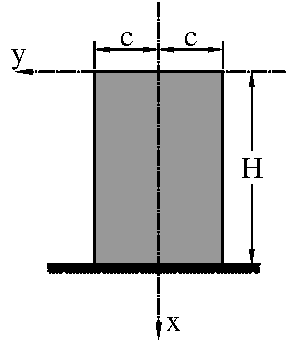
\includegraphics[height=6.0cm]{Ejer4_13_1.pdf} 
		\caption{Medio continuo}
		\label{continuo}
	\end{figure}
	%
	En las siguientes preguntas seleccione la opci\'on correcta y justifique matem\'aticamente su selecci\'on:
	\begin{enumerate}
	  
		\item El cuerpo se encuentra en equilibrio a nivel diferencial si:
		%	
		\begin{enumerate}
		%  	
		\item La fuerza de cuerpo en la direcci\'on $y$ es $p$
		\item No hay fuerzas de cuerpo
		\item La fuerza de cuerpo en la direcci\'on $x$ es $q$
		\item La fuerza de cuerpo en la direcci\'on $x$ es $p x$.
		\item La fuerza de cuerpo en la direcci\'on $x$ es $p$.
		%	
		\end{enumerate}
		\item El vector de tracciones sobre la cara $y = c$ en el sistema de referencia $xy$ est\'a dado por: \\
		%
		\begin{enumerate}
		% 	
		\item 	%
		$[t] = \left[ \begin{array}{ccc}
		\dfrac{q}{8c^3} (2x^3c - 4xc^3 + \dfrac{12}{5}c^3x) - px \\ 
		-qx \\
		\end{array}  \right] $\\
		\item 	%
		$[t] = \left[ \begin{array}{ccc}
		-qx \\ 
		0 \\
		\end{array}  \right] $\\
		\item 	%
		$[t] = \left[ \begin{array}{ccc}
		0 \\ 
		-qx \\
		\end{array}  \right] $\\
		\item 	%	
		$[t] = \left[ \begin{array}{ccc}
		- \dfrac{q}{8c^3} (2x^3c - 4xc^3 + \dfrac{12}{5}c^3x) - px \\ 
		qx \\
		\end{array}  \right] $\\	
		\item Ninguna de las anteriores.
		%	
		\end{enumerate}\	
		
		\item La magnitud de la fuerza en direccion $y$ que actua en la cara $y = c$ es:\\
	%	%
		\begin{enumerate}
	%	% 	
		\item $F = q H^2 $.\\
		\item $F = \dfrac{q H^2}{2} $. \\
		\item $F = 2 q c $. \\
		\item $F = \dfrac{q H}{2} $. \\
		\item Ninguna de las anteriores.
		%	
		\end{enumerate}	
	
		\item Si el tensor $[\sigma]$ se emplea como la soluci\'on de esfuerzos para la presa mostrada en la \cref{presa}, seleccione cual de las siguientes afirmaciones es correcta. \\
	%
	\begin{figure}[H]
		\centering
		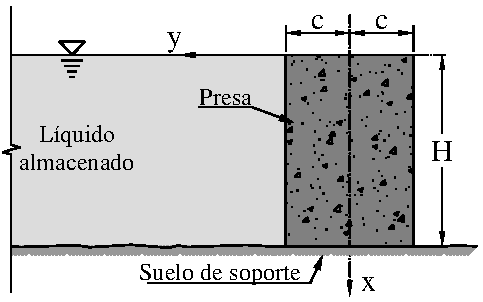
\includegraphics[height=6cm]{Ejer4_13_2.pdf} 	
		\caption{Presa}
		\label{presa}
	\end{figure}
	%
		\begin{enumerate} 
			\item El tensor satisface plenamente las condiciones de frontera en todas las caras (y = c, y = -c, x = 0, x = H).
			\item El tensor satisface plenamente las condiciones de frontera en las caras y = c y x = 0.
			\item El tensor no satisface las condiciones de frontera en la cara y = -c.
			\item El tensor no satisface las condiciones de frontera en la cara x = 0.
			\item Ninguna de las afirmaciones es correcta.
		\end{enumerate}

		\item Aceptando como soluci\'on el tensor presentado en el numeral [1] y considerando que la presa est\'a construida con suelo compactado cuya resistencia ante esfuerzo cortante es de $ 0.5 \dfrac{kgf}{cm^2}$; si H = 3.0 m, c = 1.1 m, q = 1000 $\dfrac{kgf}{m^3}$ y p = 2000 $\dfrac{kgf}{m^3}$ se puede afirmar:
		%
		\begin{enumerate} 
	%		\item[a] La presa no fallar\'ia ante esfuerzos de corte en el plano $xy$ porque el cortante m\'aximo es menor 0.5 $\dfrac{kgf}{cm^2}$
			\item La presa fallar\'ia ante esfuerzos de corte en el plano $xy$ porque el cortante en el punto de coordenadas (3.0 m,1.1 m) es mayor a 0.5 $\dfrac{kgf}{cm^3}$
			\item La presa fallar\'ia ante esfuerzos de corte en el plano $xy$ porque la magnitud del cortante m\'aximo en el punto de coordenadas (0.0 m,-1.1 m) es mayor a 0.5 $\dfrac{kgf}{cm^2}$. 
			\item La presa no fallar\'ia ante esfuerzos de corte en el plano $xy$ porque la magnitud del cortante m\'aximo en el punto de coordenadas (3.0 m,0.0 m) es menor a 0.5 $\dfrac{kgf}{cm^2}$. 
			\item La presa fallar\'ia ante esfuerzos de corte en el plano $xy$ porque la magnitud del cortante m\'aximo en el punto de coordenadas (3.0 m,-1.1 m) es mayor a 0.5 $\dfrac{kgf}{cm^2}$
		%	
		\end{enumerate}\	
	\end{enumerate}
% *************************** %
\item \label{punto14} En la figura \ref{viga:voladizo} se muestra un cuerpo de
secci\'on rectangular de ancho unitario, altura $H$, soportado en un extremo ($X = 0$), y sometido en su otro extremo ($X = L$) a la acci\'on de una fuerza $P$ en la direcci\'on Y. Si el tensor de esfuerzos en el sistema coordenado $XYZ$ est\'a dado por:\\
\\
%
	$\sigma_{xx} = - \dfrac{P}{I} (XY)$ \hspace{40mm} $\sigma_{yy} = \sigma_{zz} = 0$ \\\\	
	$\tau_{xy} = \tau_{yx} = - \dfrac{P}{2I} (\dfrac{H^2}{4} - Y^2) $\hspace{20mm} $\tau_{xz} = 0$ \\	
%
Donde $I$ es el momento de inecia de la secci\'on respecto a el eje Z y P es la fuerza.
\begin{figure}[H]
	\centering
	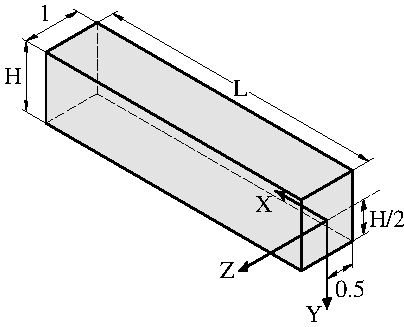
\includegraphics[height=6cm]{Ejer4_14.pdf} 
	\caption{Viga en volodizo}
	\label{viga:voladizo}
\end{figure}
%
	\begin{enumerate}
		\item Verifique equilibrio diferencial.
		\item Verifique las condiciones de frontera.
		\item \textquestiondown Las condiciones de frontera coinciden con las presentadas en el enunciado del problema?. De ser afirmativa o negativa su respuesta, justif\'iquela.
		\item Verifique equilibrio global.
		\item \textquestiondown Cual es el valor del esfuerzo cortante m\'aximo y en donde se presenta?. 
		\item \textquestiondown Cual es el valor del esfuerzo normal m\'aximo y en donde se presenta?.
	\end{enumerate}
%
% *************************** %
\item \label{punto15} En la \cref{cargaP_a} se muestra una estructura
especial actuando sobre un cuerpo de concreto de gran dimensi\'on. El estado de esfuerzos al interior del cuerpo debidos a la acci\'on de la estructura, en un sistema coordenado cil\'indrico $(r,{\theta},z)$, est\'an dados por:\\\\
%
\begin{large}
	\hspace*{10mm}$\sigma_{rr}= -\dfrac{2Q}{\pi r} Cos \theta$; \hspace*{5mm}
	$\sigma_{\theta\theta} = \sigma_{zz} = 0$; \hspace*{5mm}
	$\tau_{r\theta}= \tau_{rz}= 0 $; \hspace*{5mm}
	$\tau_{\theta{z}} = \dfrac{Q}{\pi r} \sqrt{3}$ \\\\
\end{large}
%
$Q$ es una constante positiva, $r$ es la distancia desde la ubicaci\'on de la estructura al punto de evaluaci\'on y $\theta$ es el \'angulo medido desde la horizontal en sentido antihorario. 
%
\begin{figure}[H]
	\centering
		\subfloat [Solución fundamental ]{ 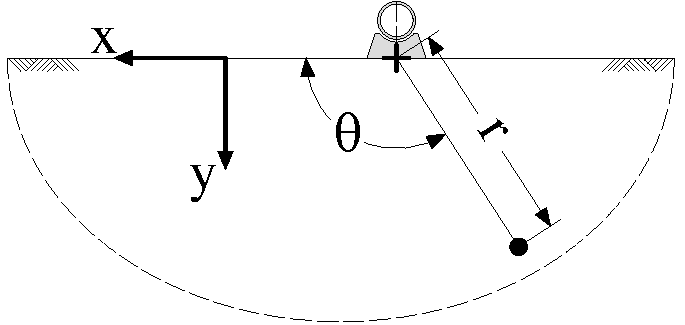
\includegraphics[width=2.6in]{Ejer4_15_1.pdf}\label{cargaP_a}}
		\hspace{1.0cm}
		\subfloat [Estructuras y cable]{ 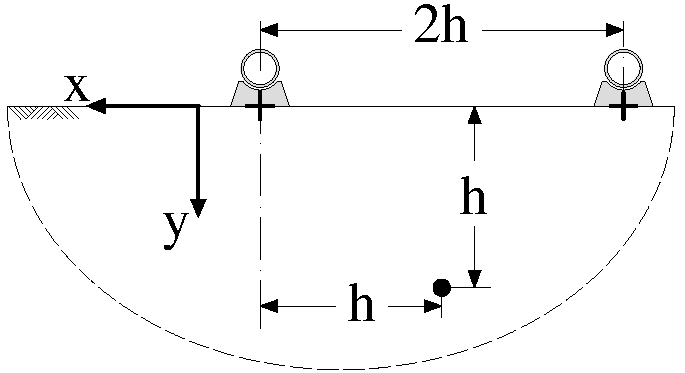
\includegraphics[width=2.6in]{Ejer4_15_2.pdf}\label{cargaP_b}}		
	%\caption{Estructuras sobre la superficie}
	\label{cargaP_concreto} 
\end{figure}
%
Si se desea instalar un cable (de d\'iametro despreciable) perpendicular al plano mostrado ($XY$) a una profundidad $h = 4 \sqrt{2}$ y se sabe que el cuerpo está sometido a la 
 la acci\'on de dos estructuras iguales, tal como se muestra en la \cref{cargaP_b}. Determine: \\

\begin{enumerate}
	% 
	\item Si el cable es infinitamente resistente ante esfuerzos normales pero
	{\textbf {\large{$\tau_{crit}$}}} es el m\'aximo esfuerzo de corte que resiste, \textquestiondown cu\'al es el m\'aximo valor de la carga $Q$ que pueden transmitir las estructuras para que el cable no falle?.
	%
	\item Si {\textbf {\large{$\tau_{crit}=10$}}}, \textquestiondown cu\'al es el
	valor de $Q$?.
	%
	\item Si $Q=5$, \textquestiondown cu\'al es el valor m\'inimo de {\textbf
	{\large{$\tau_{crit}$}}} para que el cable no falle por corte?.
	%
\end{enumerate}

\item  \label{punto16}   En las \cref{SolucionP} y \cref{Solucionw} se muestra las soluciones para una masa de suelo sometido a una carga superficial $P$ y una carga distribuida uniforme superficial $w$ .  Los esfuerzos al interior del suelo debidos a la carga $P$ y $w$, en un sistema  coordenado cilíndrico $\left(r,{\theta},z \right)$, est\'an dados: \\\\
%
%\begin{large}
%\centering
$[\sigma]_P = -\dfrac{2P}{\pi r} \left[ \begin{array}{ccc}
\cos\theta & 0 & 0\\ 
0 & 0 & 0\\
0 & 0 & 0\\
\end{array}  \right] $
\hspace*{5mm}
$[\sigma]_w = -\dfrac{w}{\pi} \left[ \begin{array}{ccc}
\pi + 2\theta - \sin \left(2\theta \right)  & 1 -\cos \left(2\theta\right) & 0\\ 
1 - \cos \left(2\theta \right)  & \pi + 2\theta + \sin \left(2\theta \right) & 0\\
0 & 0 & 0\\
\end{array}  \right] $
%\end{large}

Donde $P$ y $w$ son las cargas, $\theta$ es el ángulo medido desde la vertical y positivo en sentido antihorario. 
%
\begin{figure}[H]
	\centering
		\subfloat [Soluci\'on carga vertical $P$]{ 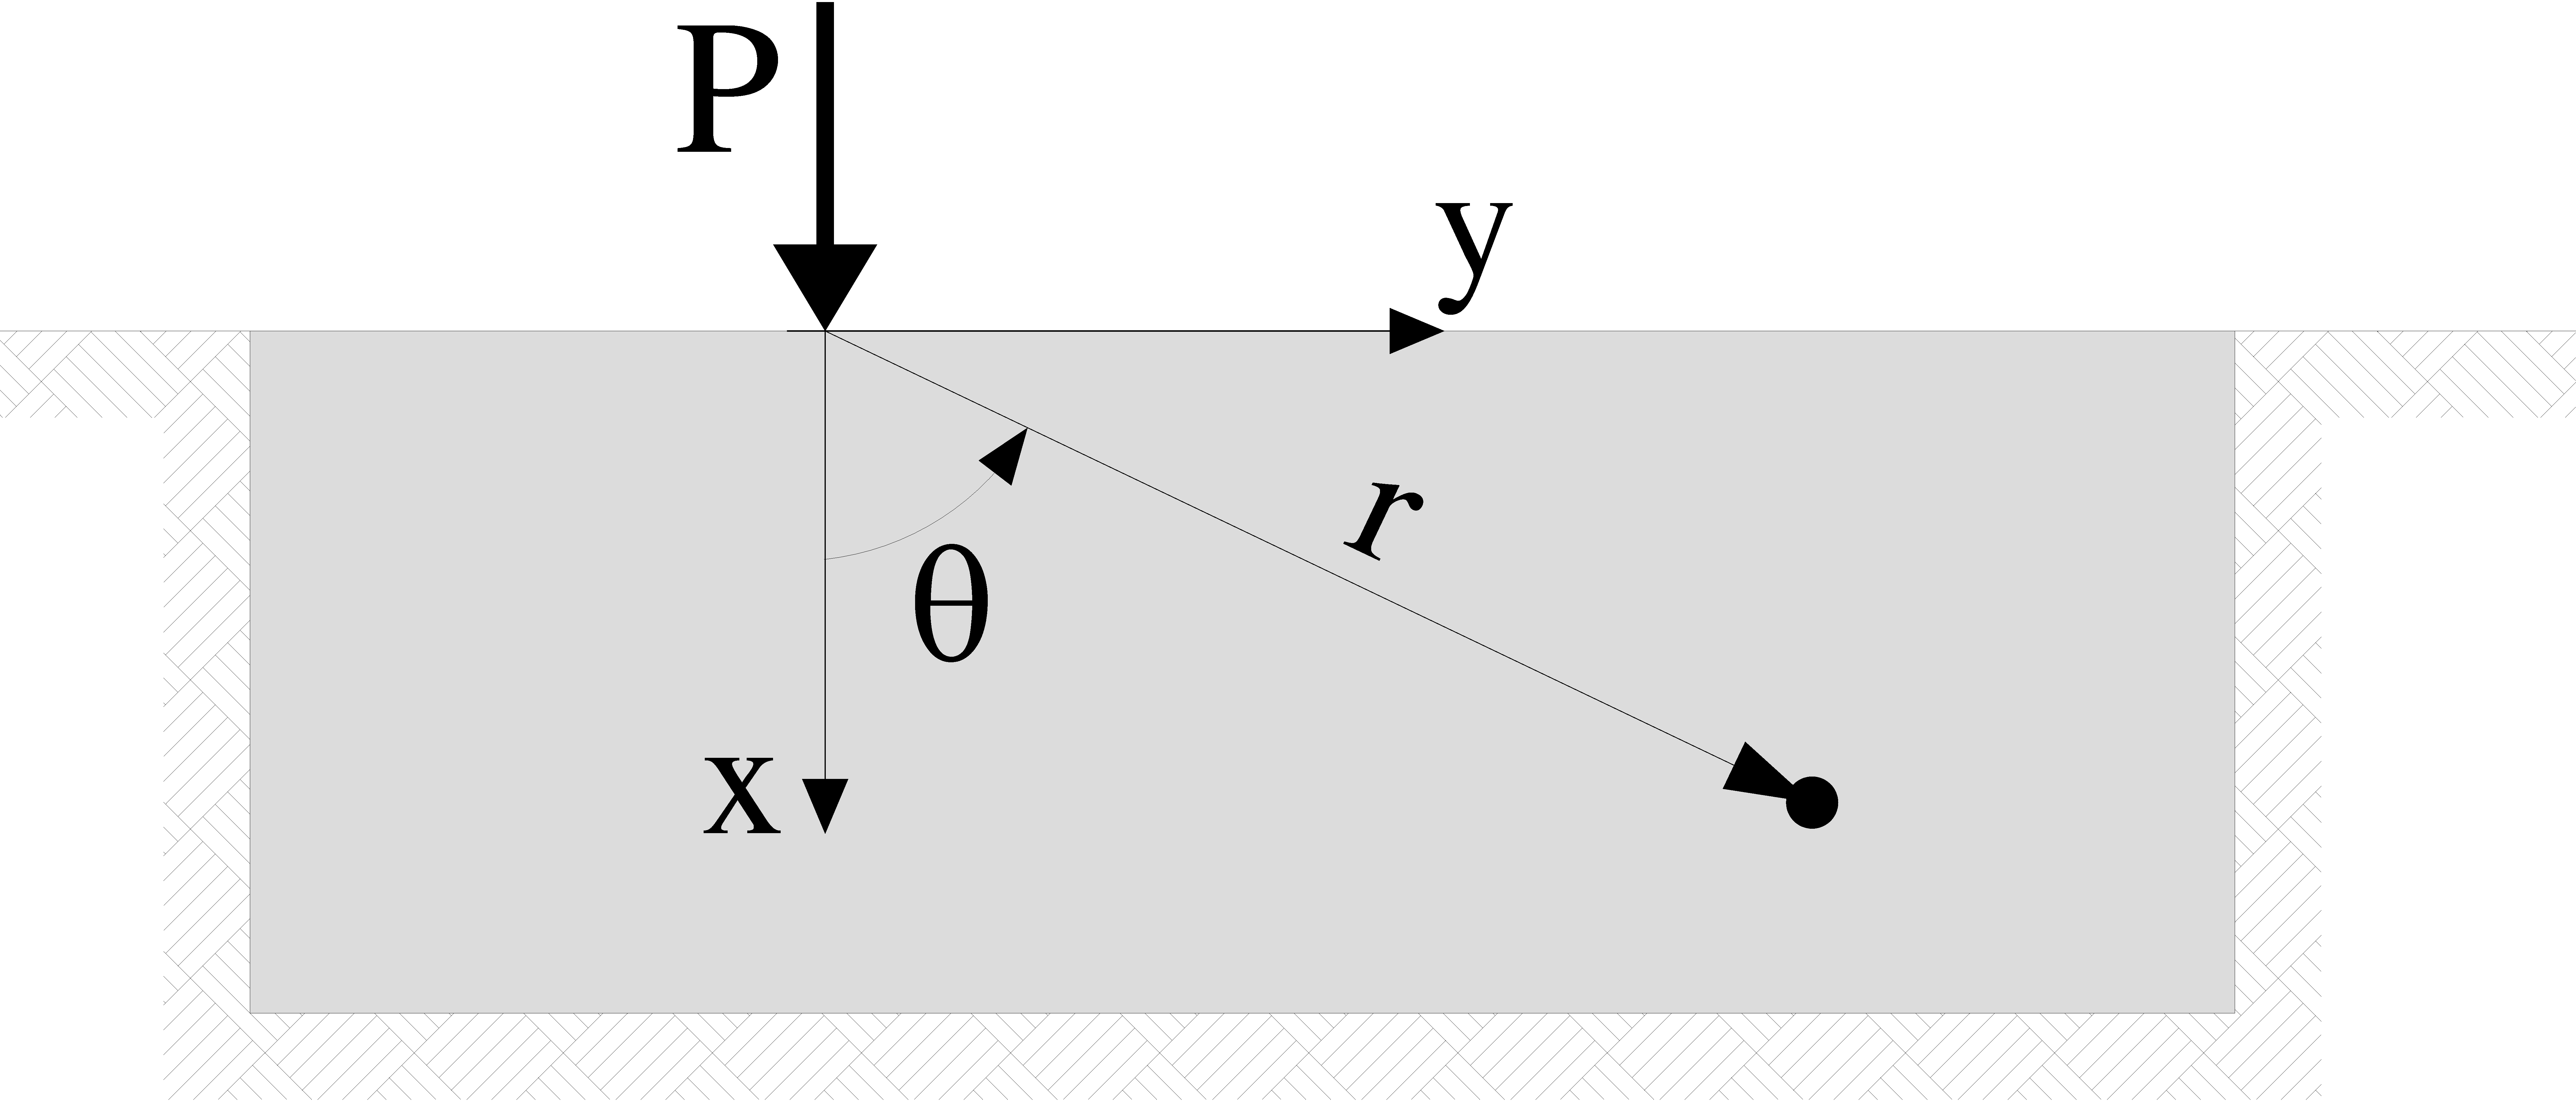
\includegraphics[width=3.0in]{Ejer4_16_1.pdf}\label{SolucionP}}
		\hspace{1.0cm}
		\subfloat [carga uniforme superficial $w$]{ 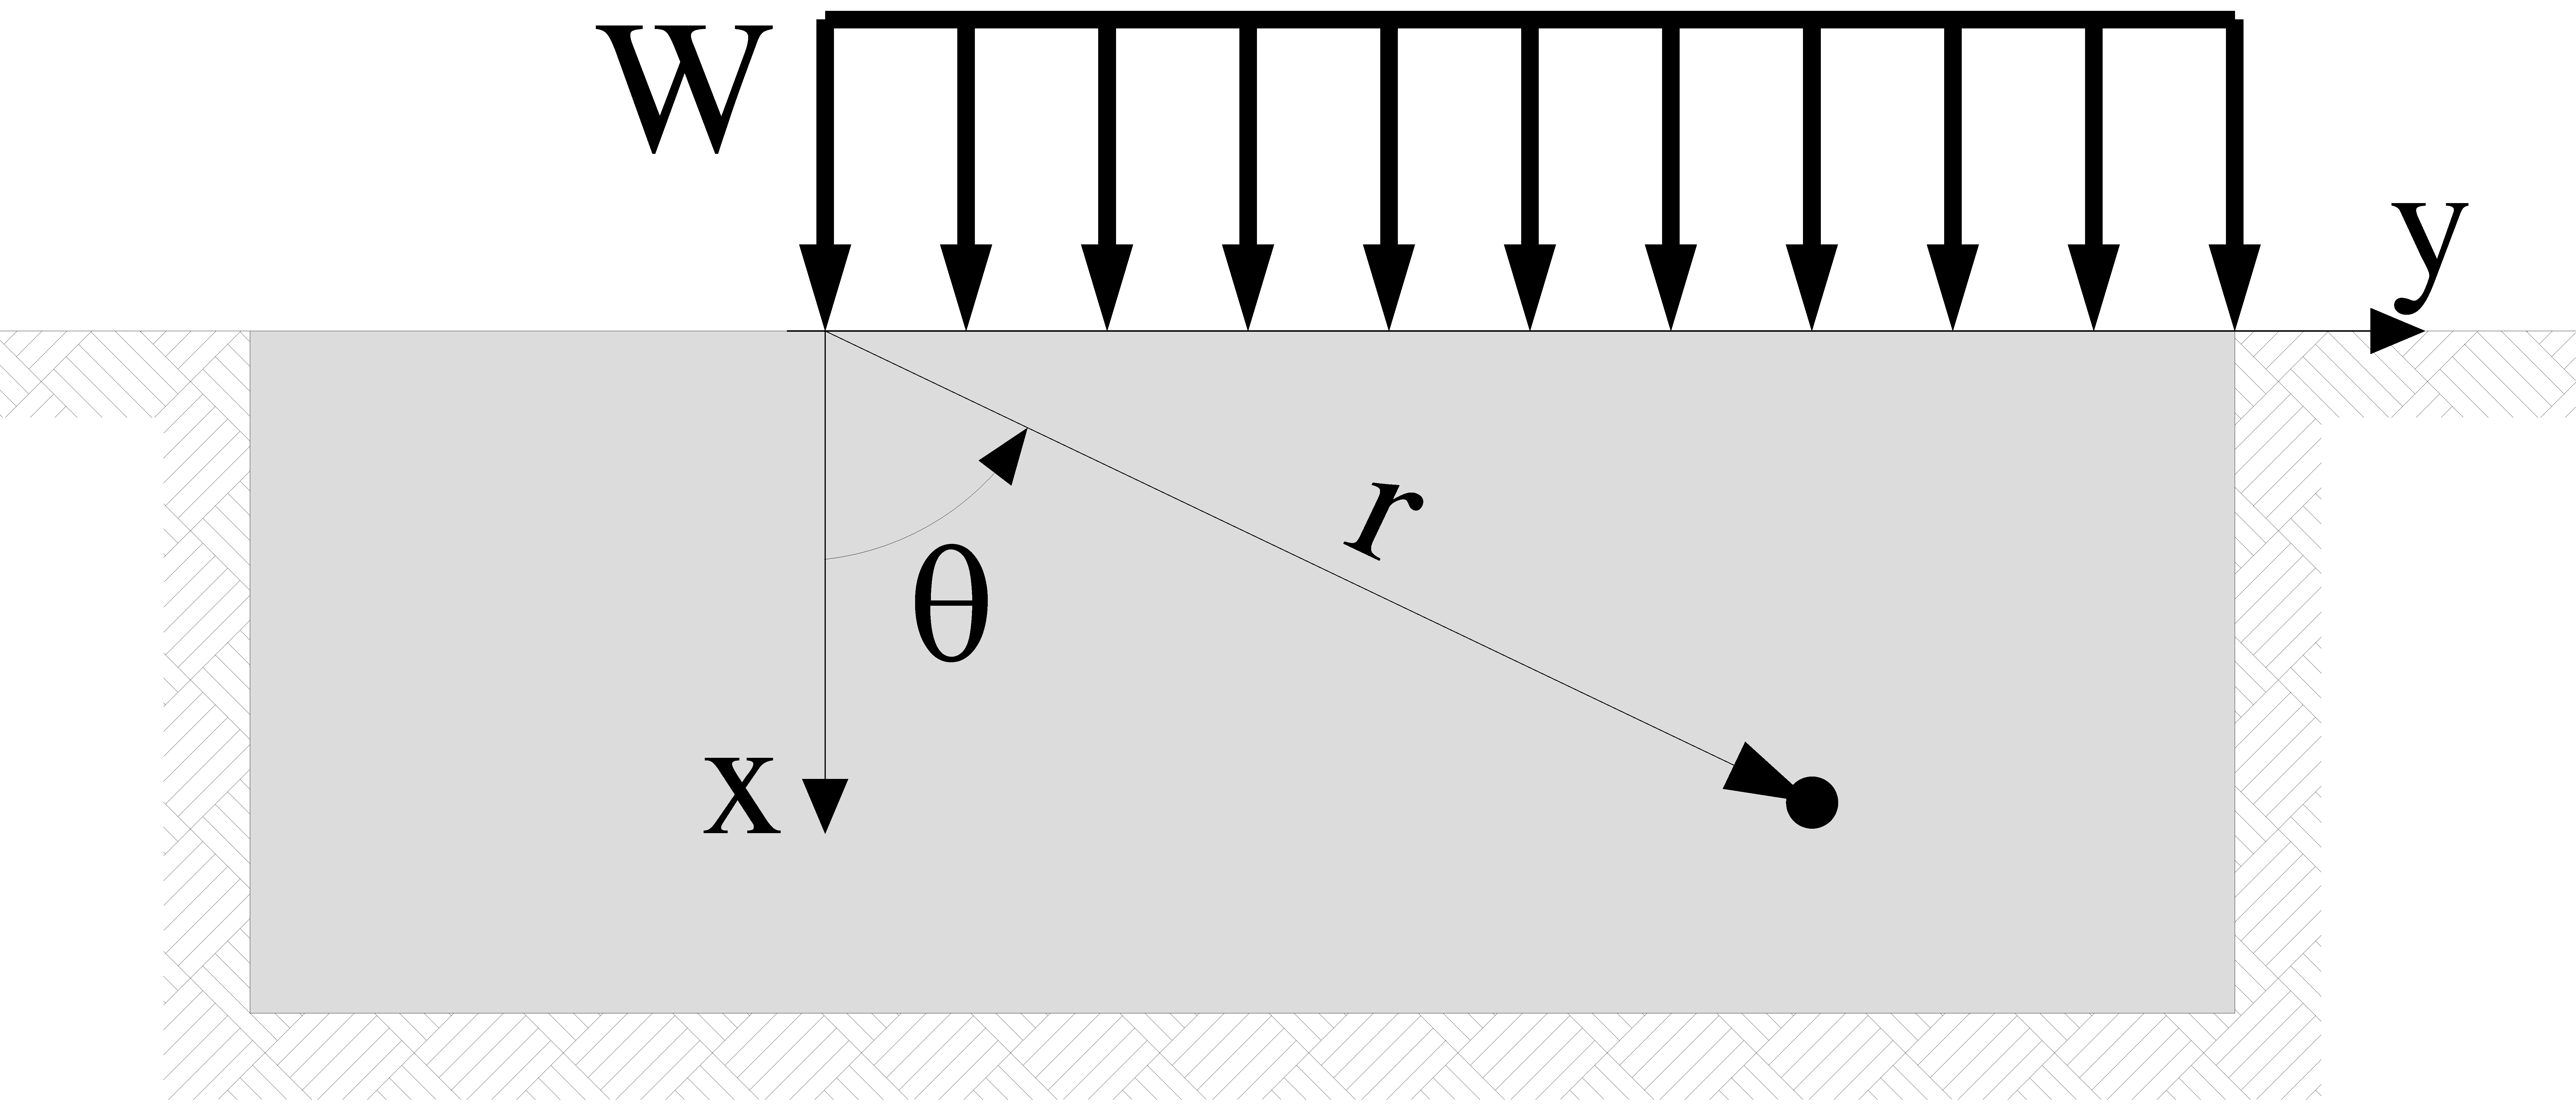
\includegraphics[width=3.0in]{Ejer4_16_2.pdf}\label{Solucionw}}		
	\caption{Soluciones fundamentales}
	\label{solucionpw} 
\end{figure}
%
Si a la masa de suelo se transmiten de manera simúltanea las cargas $P=100$ $Ton/m $ y $w= (100 + tiempo)$ $Ton/m^2$, y se quiere instalar un sistema de acueducto conformado por dos tuberías A y B (de díametro despreciable) perpendicular al plano mostrado ($XY$), en donde la profundad para la tubería A es $H_{A} = 1.0 / \pi$ $m$ y para la tubería B  es $H_{B} = 0.75 H_{A}$ tal y como se muestra en la \cref{cargasPw}. Determine:
%		
\begin{figure}[H]
	\centering
	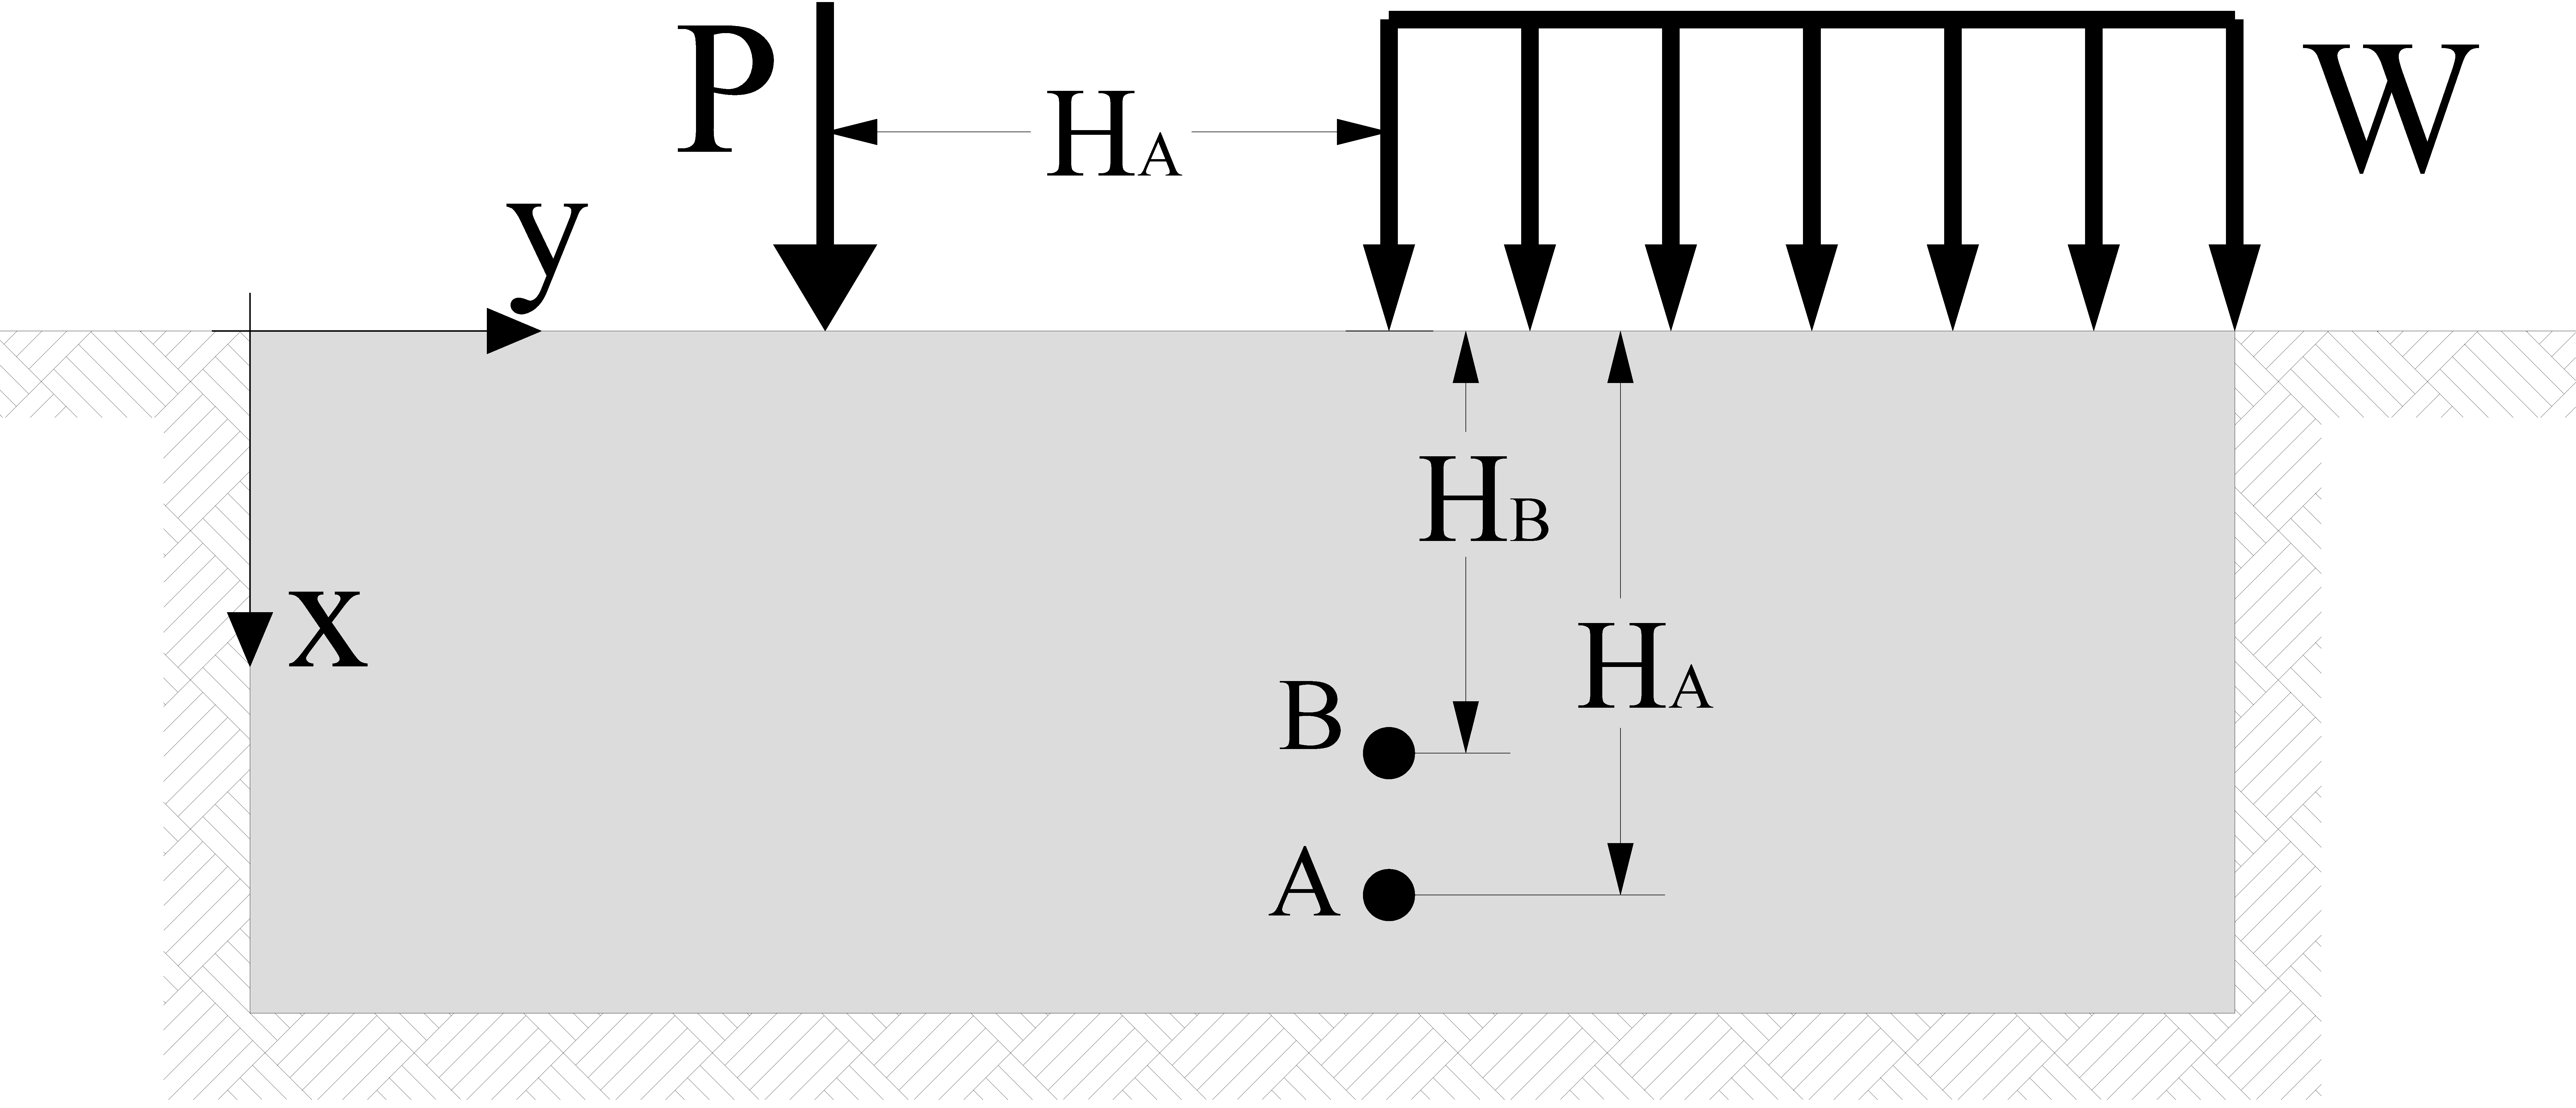
\includegraphics[width=3.5in]{Ejer4_16_3.pdf} 
	\caption{Cargas y tuber\'ias}
	\label{cargasPw}
\end{figure}
%
\begin{enumerate}
	\item  Determine cuál tubería falla primero y en que tiempo se produce la falla, si se sabe que el material de la tubería A es infinitamente resistente a esfuerzos cortantes pero no soporta esfuerzos axiales mayores o iguales a $210,5\dfrac{Ton}{m^2}$  y el material de la tubería B es infinitamente resistente a esfuerzos axiales pero no sorporta esfuerzos cortantes mayores o iguales a $100,25\dfrac{Ton}{m^2}$. 
\end{enumerate}
\newpage
\item \label{punto17}  En la \cref{barra} se presenta una barra de radio $C$ y longitud $L$. El estado de esfuerzos del  medio continuo en el sistema cartesiano $x,y,z$ est\'a dado por el tensor: \\\\
%
\begin{equation}
\begin{aligned}
& \sigma_{xx} = 0; \hspace*{5mm}  \sigma_{yy} = 0; \hspace*{5mm}  \sigma_{zz} = 0; \\
&\tau_{xy} = 0; \hspace*{5mm}  \tau_{xz} = {\omega}y;	\hspace*{5mm} \tau_{zy} = - {\omega}x \\
\end{aligned}
\label{trans}
\end{equation}
%
\begin{figure}[H]
	\centering
	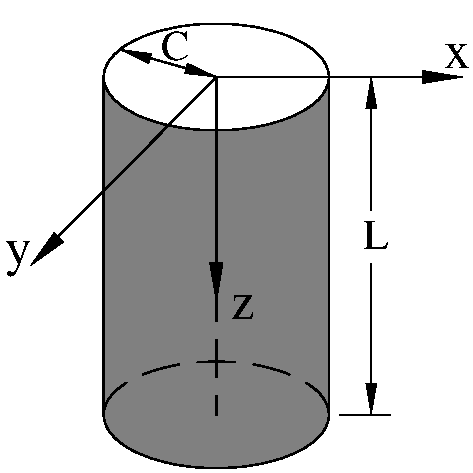
\includegraphics[height=5cm]{Ejer4_17.pdf} 
	\caption{Medio Continuo}
	\label{barra}
\end{figure}
%
Donde $\omega$ es una constante.\\
\begin{enumerate}
	\item  Determine el valor del m\'aximo esfuerzo de compresi\'on al que está sometido la barra y la ubicaci\'on (coodenadas de los puntos) donde se presentan esos valores máximos. 
    \item ¿Describa que problema resuelve el estado de esfuerzos en a barra?  \textsl{Sugerencia: para facilitar el an\'alisis estudie las caras con vector normal en direcci\'on z.} 
	\item Si el cuerpo tiene longitud $L = 50 cm$, $\omega = 5000 \; Tonf / m^3$, adem\'as es infinitamente resistente ante esfuerzos de tracci\'on y de compresi\'on, pero su capacidad m\'axima ante esfuerzos tangenciales es  $ \tau_{max} = 88 \; kgf/cm^2$.  Determine el valor m\'aximo del radio $C$ que podr\'ia tener el cuerpo. 
\end{enumerate}

\item \label{punto18}	 Si a la barra del punto \cref{punto17} adicionamente le quisieramos considerar el efecto del peso propio $\gamma$ y sabemos que el tensor de esfuerzos en el sistema coordenado $x,y,z$ en cualquier punto de los planos $z = L/3$ y $z = 2L/3$ (ver figura \ref{barrapeso}) debido solo a este efecto est\'a dado por:\\\\
%
$Puntos_{(z=L/3)}$: $[\sigma] = \left[ \begin{array}{ccc}
0 & 0 & 0\\ 
0 & 0 & 0\\
0 & 0 & 2 \gamma L/3\\
\end{array}  \right] $
\hspace{1cm}
$Puntos_{(z=2L/3)}$: $[\sigma] = \left[ \begin{array}{ccc}
0 & 0 & 0\\ 
0 & 0 & 0\\
0 & 0 & \gamma L/3\\
\end{array}  \right] $
%
\\\\\\
$\gamma = \rho g$, $\rho$ es la densidad y $g$ la gravedad. 
\begin{figure}[H]
	\centering
	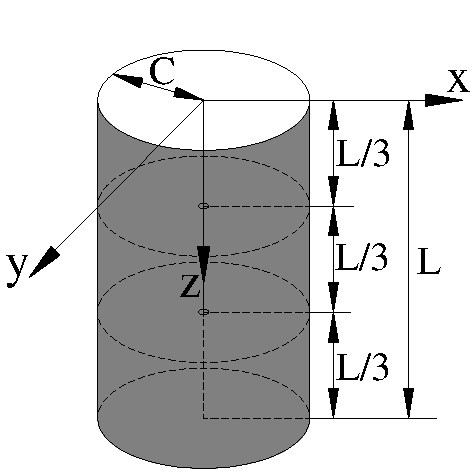
\includegraphics[height=5cm]{Ejer4_18.pdf} 
	\caption{Funci\'on peso propio}
	\label{barrapeso}
\end{figure}
% 
Adem\'as dicho esfuerzo es descrito por una funci\'on lineal en z.
 \\
\begin{enumerate}
	\item Si se tiene en cuenta que estado final de esfuerzos es la suma de estados individuales, determine cu\'al es el tensor de esfuerzos del problema  que considera conjuntamente el tensor de esfuerzos del \cref{punto18} y el peso propio. 
	\item Diga si el cuerpo est\'a o no en equilibrio diferencial (local) est\'atico. S\'i es del caso, de una propuesta para lograr dicho equilibrio. Justifique su respuesta matem\'aticamente\\  
\end{enumerate}
%	
\item \label{punto19}	 El estado de esfuerzos en un punto de un medio continuo est\'a dado por: \\
 \\
	\hspace*{10mm} $ \sigma_{xx} (t)= K(t)$; \hspace*{5mm} $\sigma_{yy} (t) = -6K(t)$;\hspace*{5mm} $ \sigma_{zz} (t)= -K(t)$; \\\\
	\hspace*{10mm} $ \tau_{xy} (t) = 0$; \hspace*{5mm} $\tau_{xz} (t) = 0$; \hspace*{5mm} $\tau_{yz} (t) = 0$ \\
\\	
Donde, $K(t)$ es un par\'ametro que var\'ia en funci\'on del tiempo $t$, tal como se muestra en la gráfica y tabla presentadas en la \cref{fig:esfuerzo_dependiente_tiempo}.
\begin{minipage}{0.3\textwidth}
\begin{tabular}{cc}
$t$ (s) & $K(t)$ (kgf/cm$^2$) \\ 
\hline\\
0.0 & 2.0 \\ 
5.0 & 2.0 \\ 
10.0 & 4.0 \\ 
15.0 & 0.0 \\ 
20.0 & -6.0 \\  
25.0 & 0.0\\
\end{tabular} 
\end{minipage}
\begin{minipage}{0.6\textwidth}
\begin{figure}[H]
  \centering
  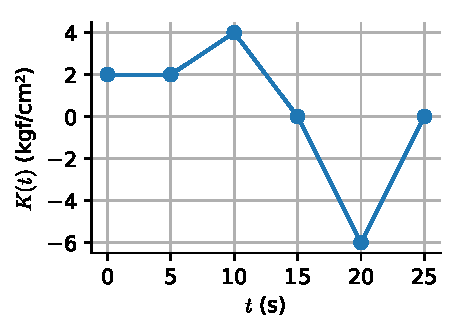
\includegraphics[width=3 in]{esfuerzo_dependiente_tiempo.pdf} 	
  \caption{Variación del parámetro $K$}
  \label{fig:esfuerzo_dependiente_tiempo}
\end{figure}
\end{minipage}


\begin{enumerate}
	\item Si el material es infinitamente resistente ante esfuerzos normales (axiales), pero no soporta esfuerzos cortantes mayores o iguales a $13\dfrac{kgf}{cm^2}$ determine el instante en que se presenta la falla en caso de que se presente. Si no hay falla ind\'iquelo claramente.
\end{enumerate}
\item \label{punto20} En la figura \ref{dona} se presenta la secci\'on
transversal de un cilindro. Los esfuerzos en el dominio est\'an representados por:\\\\
	\\
	$\sigma_{r} = \dfrac{a^2 b^2 (p_o-p_i)}{(b^2-a^2)r^2} + \dfrac{p_i a^2 - p_o b^2}{b^2-a^2}$ \hspace{10mm}
	$\sigma_{\theta} = -\dfrac{a^2 b^2 (p_o-p_i)}{(b^2-a^2)r^2} + \dfrac{p_i a^2 - p_o b^2}{b^2-a^2}$\hspace{10mm}
	$\tau_{r \theta} = 0$ 
	%
	\begin{figure}[H]
		\centering
		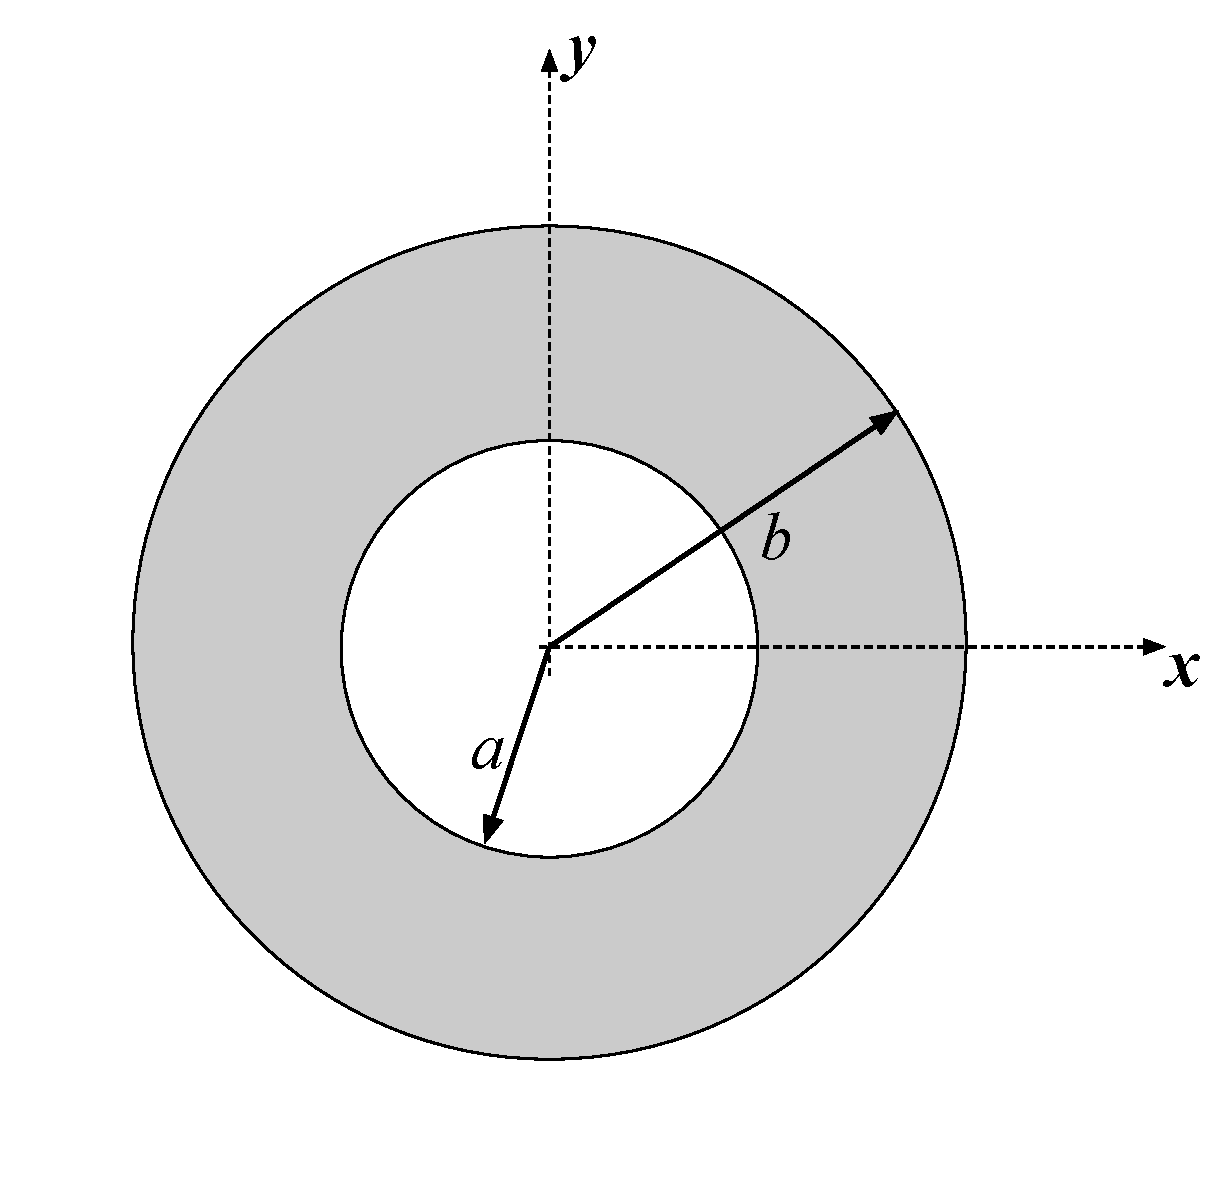
\includegraphics[height=5.5cm]{Ejer4_20.pdf} 
		\caption{Secci\'on transversal cilindro}
		\label{dona}
	\end{figure}
	%
	\begin{enumerate}
		\item Verifique el equilibrio diferencial.
		\item \textquestiondown Cuales son las cargas externas a las cuales est\'a sometido el cilindro?. Indíquelas gr\'aficamente.
		\item \textquestiondown Cual es el esfuerzo axial m\'aximo y d\'onde se presenta?.
		\item \textquestiondown Cual es el esfuezo de corte m\'aximo y d\'onde se presenta?.
	\end{enumerate}
%
\item \label{punto21} En la \cref{PtoPol} muestra el estado de tensiones en un punto de coordenadas $(X,Y) = (55/\sqrt{2},55/\sqrt{2})$  al interior de un Medio Continuo. Sobre una de las caras asociadas al eje $Y'$ se dan las tensiones $\sigma_{Y'Y'}$ y $\tau_{Y'X'}$ y sobre una de las caras asociadas al eje $X'$ se da el vector de tracciones expresado en el sistema de referencia $XY$.
%
\begin{figure}[H]
	\centering
	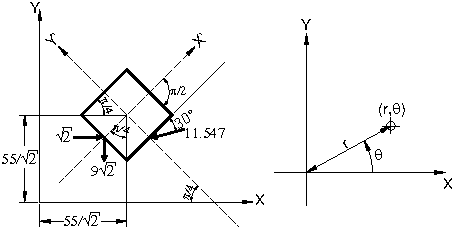
\includegraphics[height=6.25cm]{Ejer4_21.pdf} 
	\caption{Estado de tensiones en un punto al interior de un medio continuo.}
	\label{PtoPol}
\end{figure}
%
\begin{enumerate}
	\item Escribir el tensor de tensiones en el sistema de referencia polar $r,\theta$. \\
\end{enumerate}


\item \label{punto23}  Los tensores
\[[\sigma(r,{\theta})]_P
 	= 
 	\begin{bmatrix}
     	-\dfrac{2P\cos\theta}{(2\alpha + \sin(2\alpha)) r} & 0 \;\;\;\\
     	0 & 0 \;\;\;
 	\end{bmatrix}
 	\hspace{2cm}
	[\sigma(r,{\theta})]_Q
 	= 
  	\begin{bmatrix}
     	-\dfrac{2Q\sin\theta}{(2\alpha - \sin(2\alpha)) r} & 0 \;\;\; \\
     	0 & 0 \;\;\;
 	\end{bmatrix}\]
 	
representan el estado de tensiones en un punto de coordenadas $(r, \theta)$ al interior de las cuñas de semi-ángulo interno $\alpha$ (medido en radianes) mostradas en las \cref{CargaP} y \cref{CargaQ}, resultantes de la aplicación de cargas puntuales $P$ y $Q$ respectivamente. 


\begin{figure}[H]
	\centering	
	\subfloat[Cuña de semi-ángulo interno $\alpha$ sometida a una carga vertical P.]{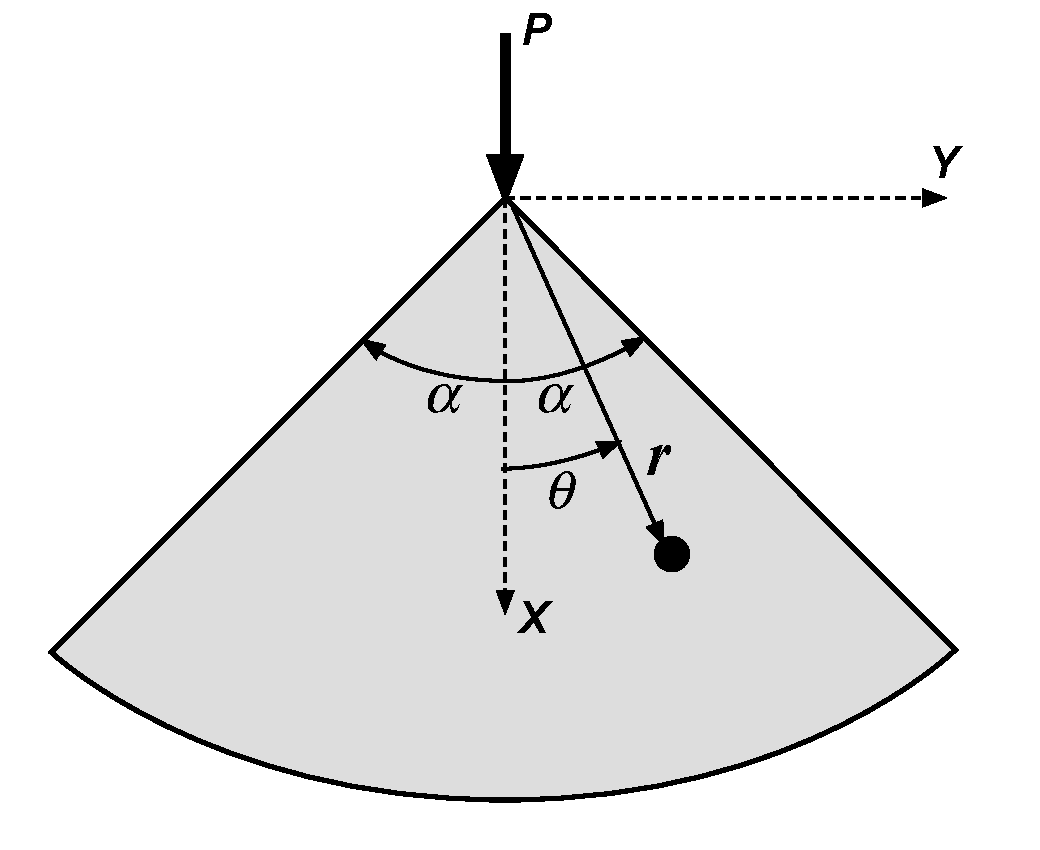
\includegraphics[width=3.0in]{figure_1b_T1.pdf}\label{CargaP}}	
	\hspace{1.5cm}
	\subfloat[Cuña de semi-ángulo interno $\alpha$ sometida a una carga vertical Q.]{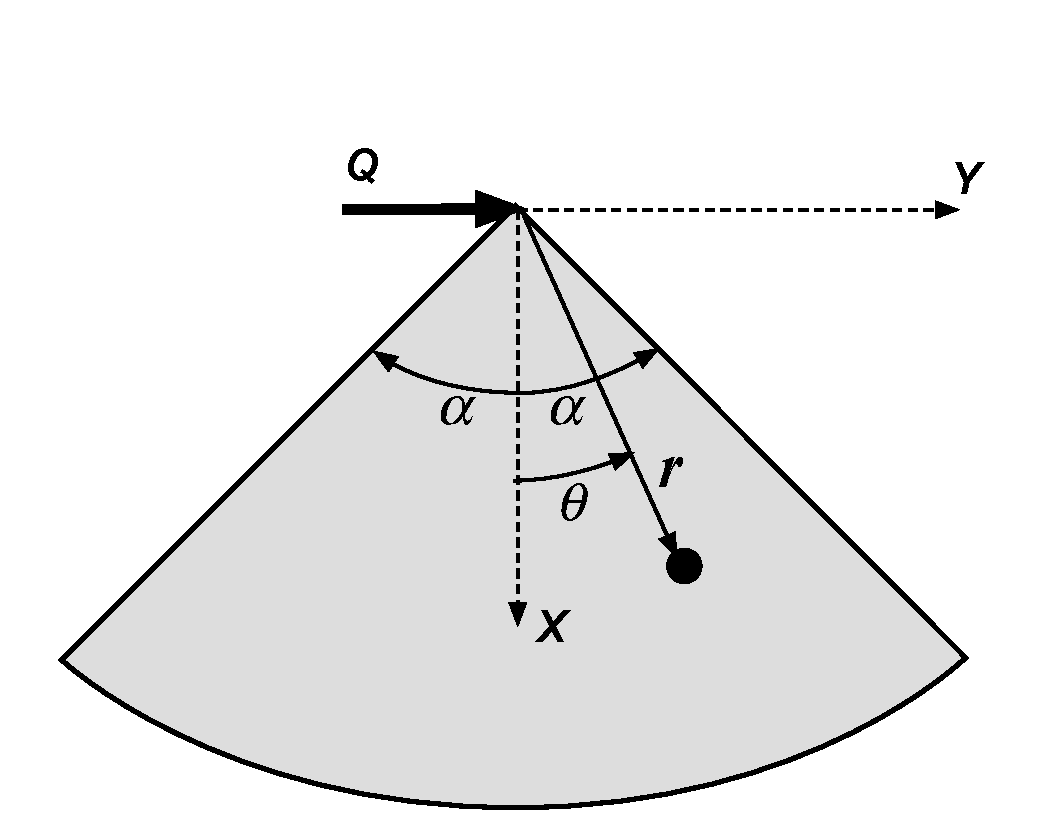
\includegraphics[width=3.0in]{figure_1c_T1.pdf}\label{CargaQ}}
	\caption{Cuña de semi-ángulo interno $\alpha$. }
%	\label{figure2}
\end{figure}

Usando dichas soluciones se pide determinar el estado de tensiones para un punto P de coordenadas $(r, \theta)$ localizado al interior de un depósito de suelo sometido a una carga puntual de magnitud $F$ como se muestra en la \cref{figure1}. 
%
\begin{figure}[h]
	\centering
		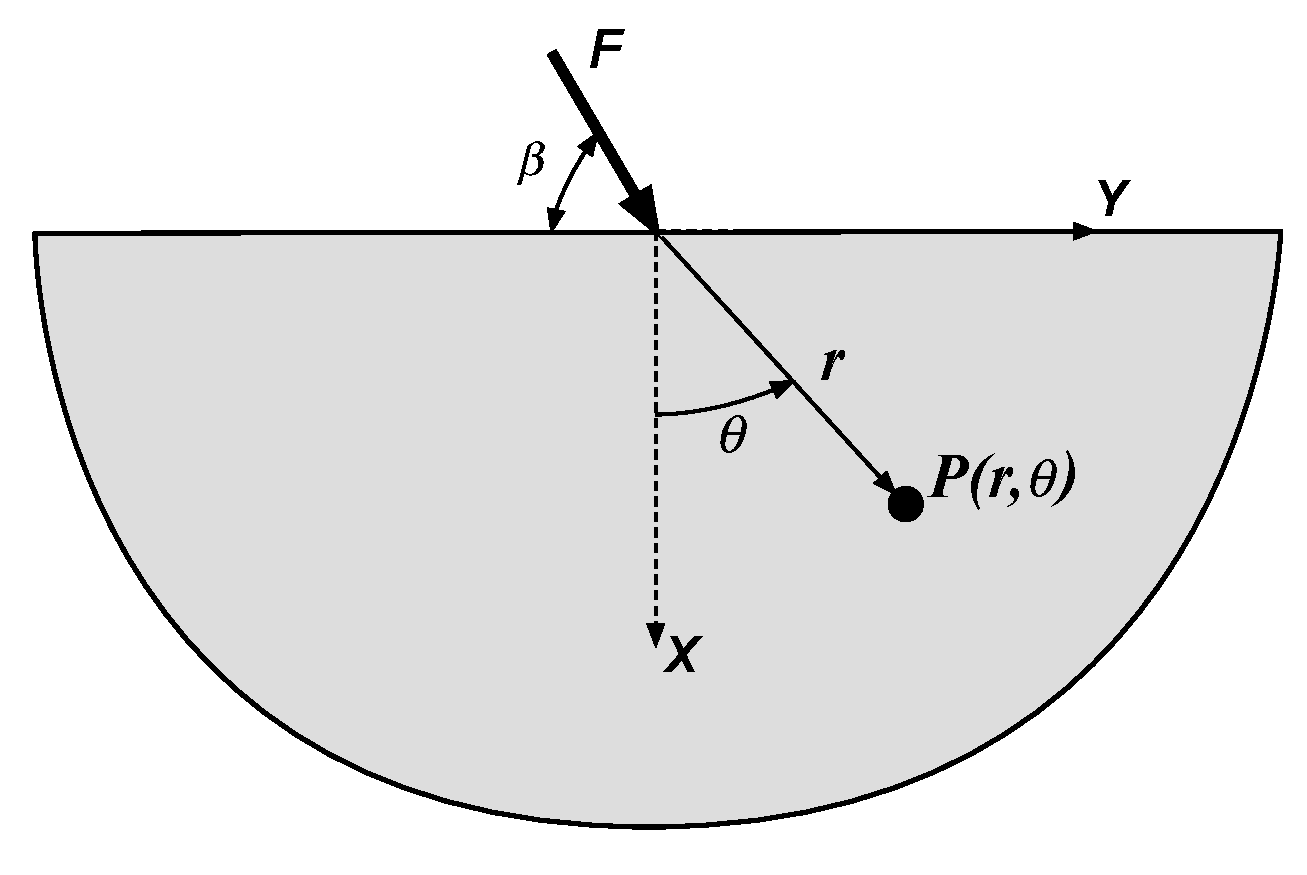
\includegraphics[width=4.0in]{figure_1a_T1.pdf} 		
	\caption{Depósito de suelo sometido a una carga puntual $F$.}
	\label{figure1}
\end{figure}
\end{enumerate}
\end{document}


